\appendix
\section{Robustness Check Details}
\label{sec:appendix}

\textbf{RC-4 (Winsorization):} \texttt{N\_tasks} winsorized at 99th percentile; refitted P1 model yields IRR$\approx$1.22 --- consistent with primary. Gate passes.

\textbf{RC-7 (Age vs.\ Decade FE):} Replacing \texttt{C(decade)} with \texttt{age\_years}-only control; \texttt{has\_tags} effect attenuates slightly but remains above 1.1 gate and $p<0.001$.

\textbf{RC-3 (Collinearity documentation):} Cram\'er's V=0.823 for decade $\times$ \texttt{has\_tags} documented; attenuation\_ratio=1.1219 confirms non-fatal. Full decade-\texttt{has\_tags} collinearity context shown in Figure~\ref{fig:decade_adoption}.

\begin{figure}[h]
\centering
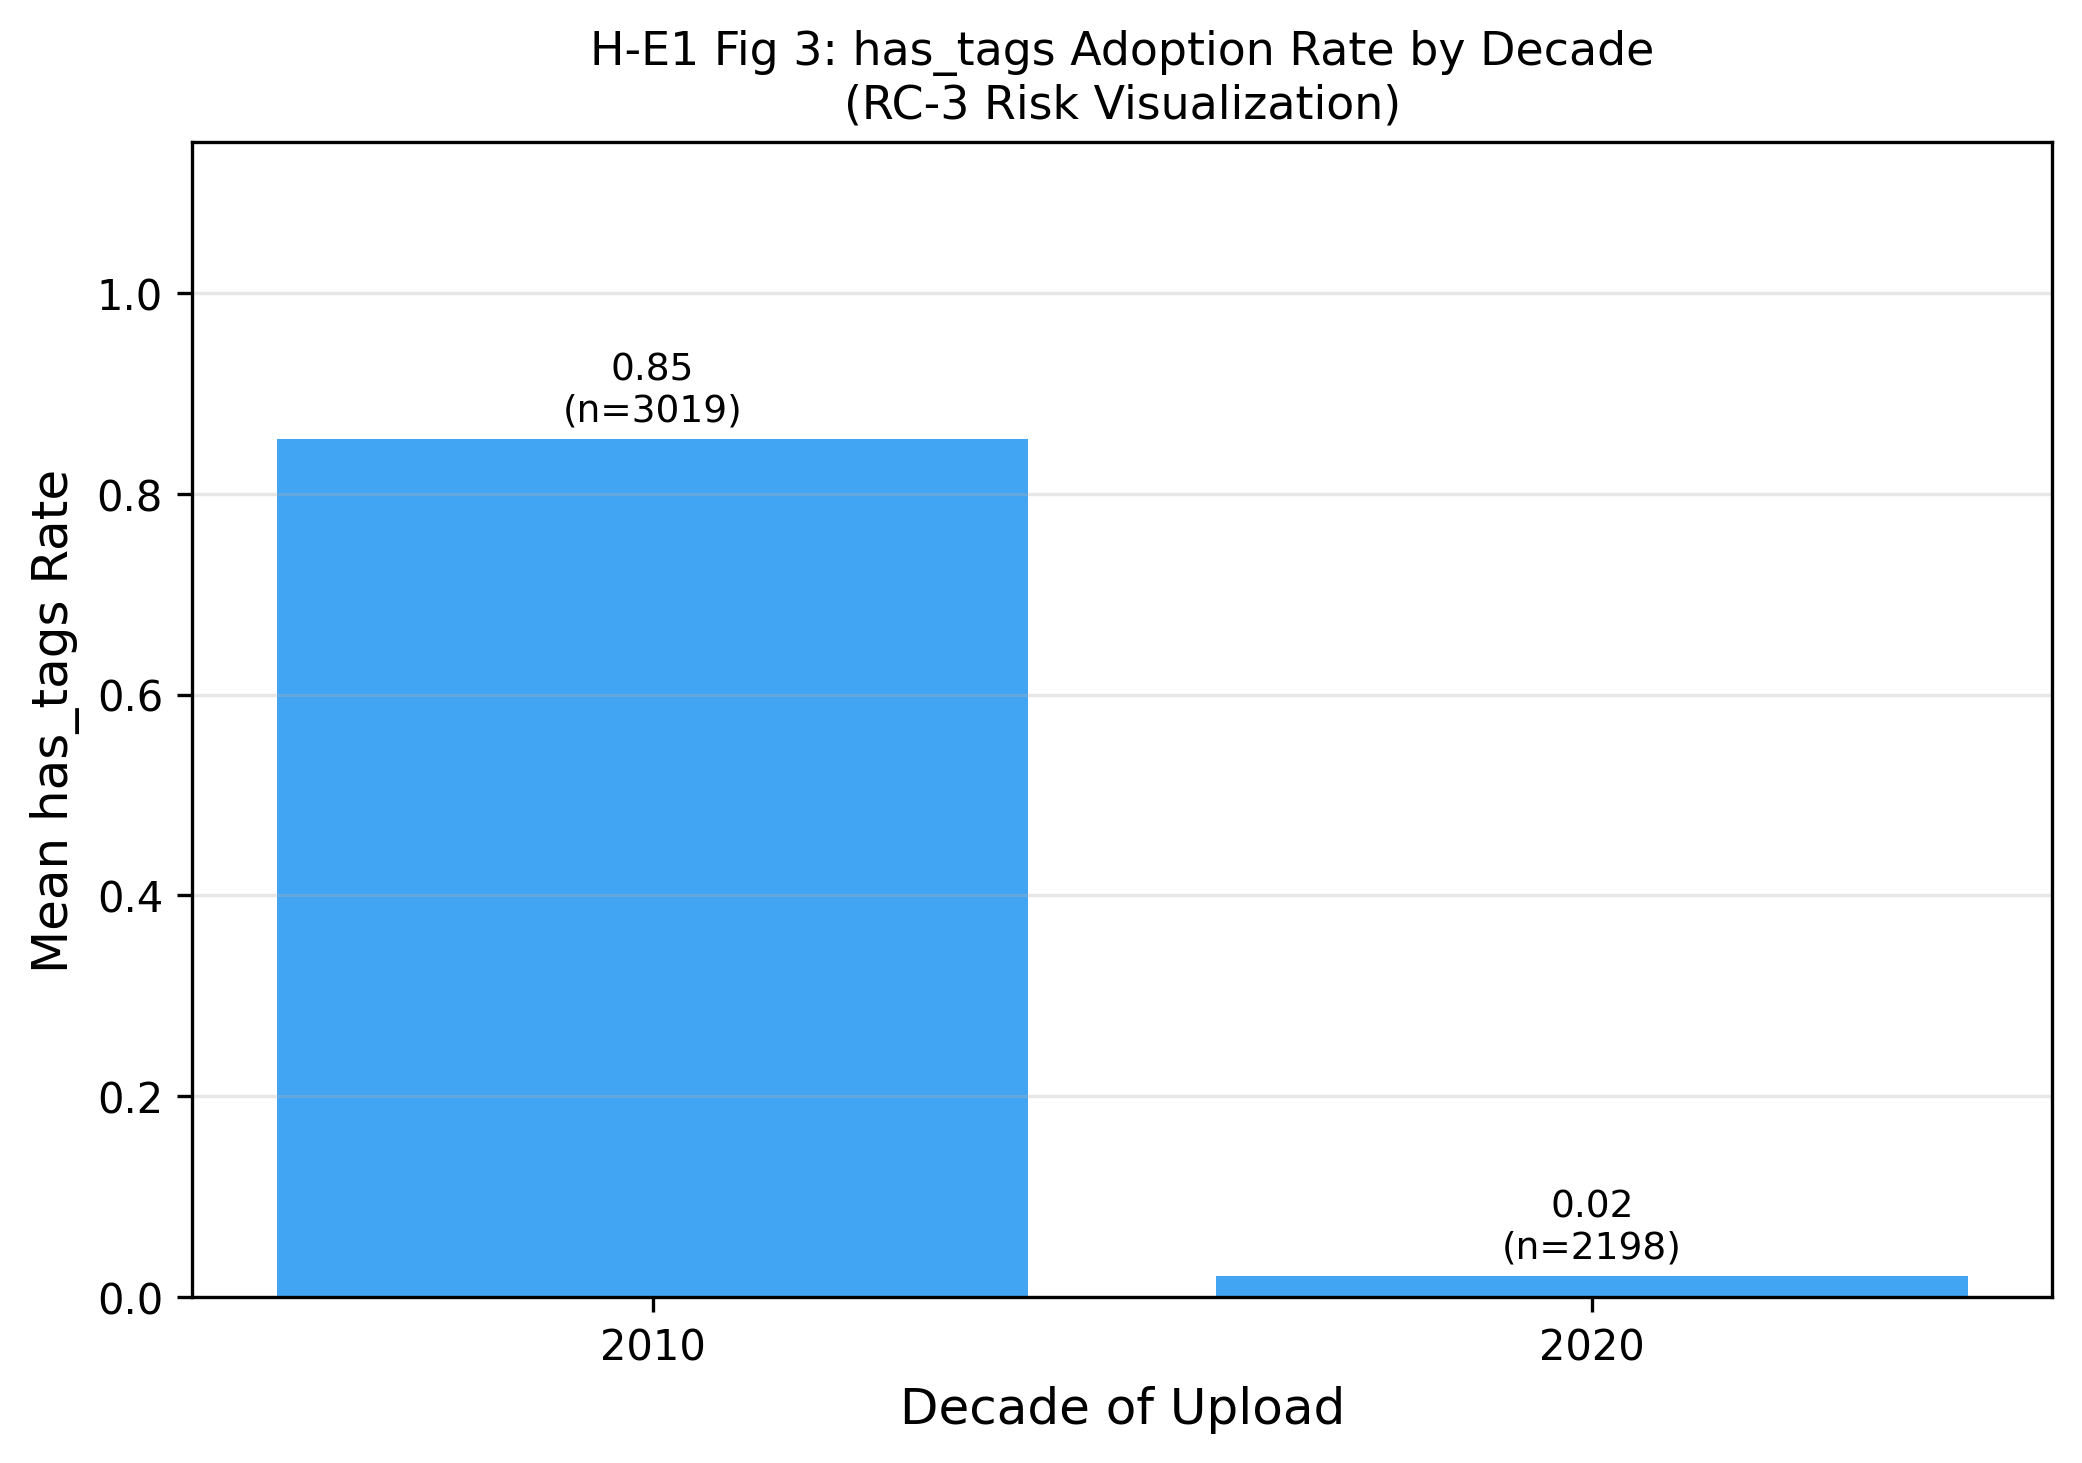
\includegraphics[width=0.65\linewidth]{figures/fig3_decade_adoption.png}
\caption{Decade-by-decade adoption patterns. Tagging prevalence increases monotonically with decade (Cram\'er's V=0.823), but the within-decade \texttt{has\_tags} effect persists across all cohorts.}
\label{fig:decade_adoption}
\end{figure}

\textbf{Model fit:}

\begin{figure}[h]
\centering
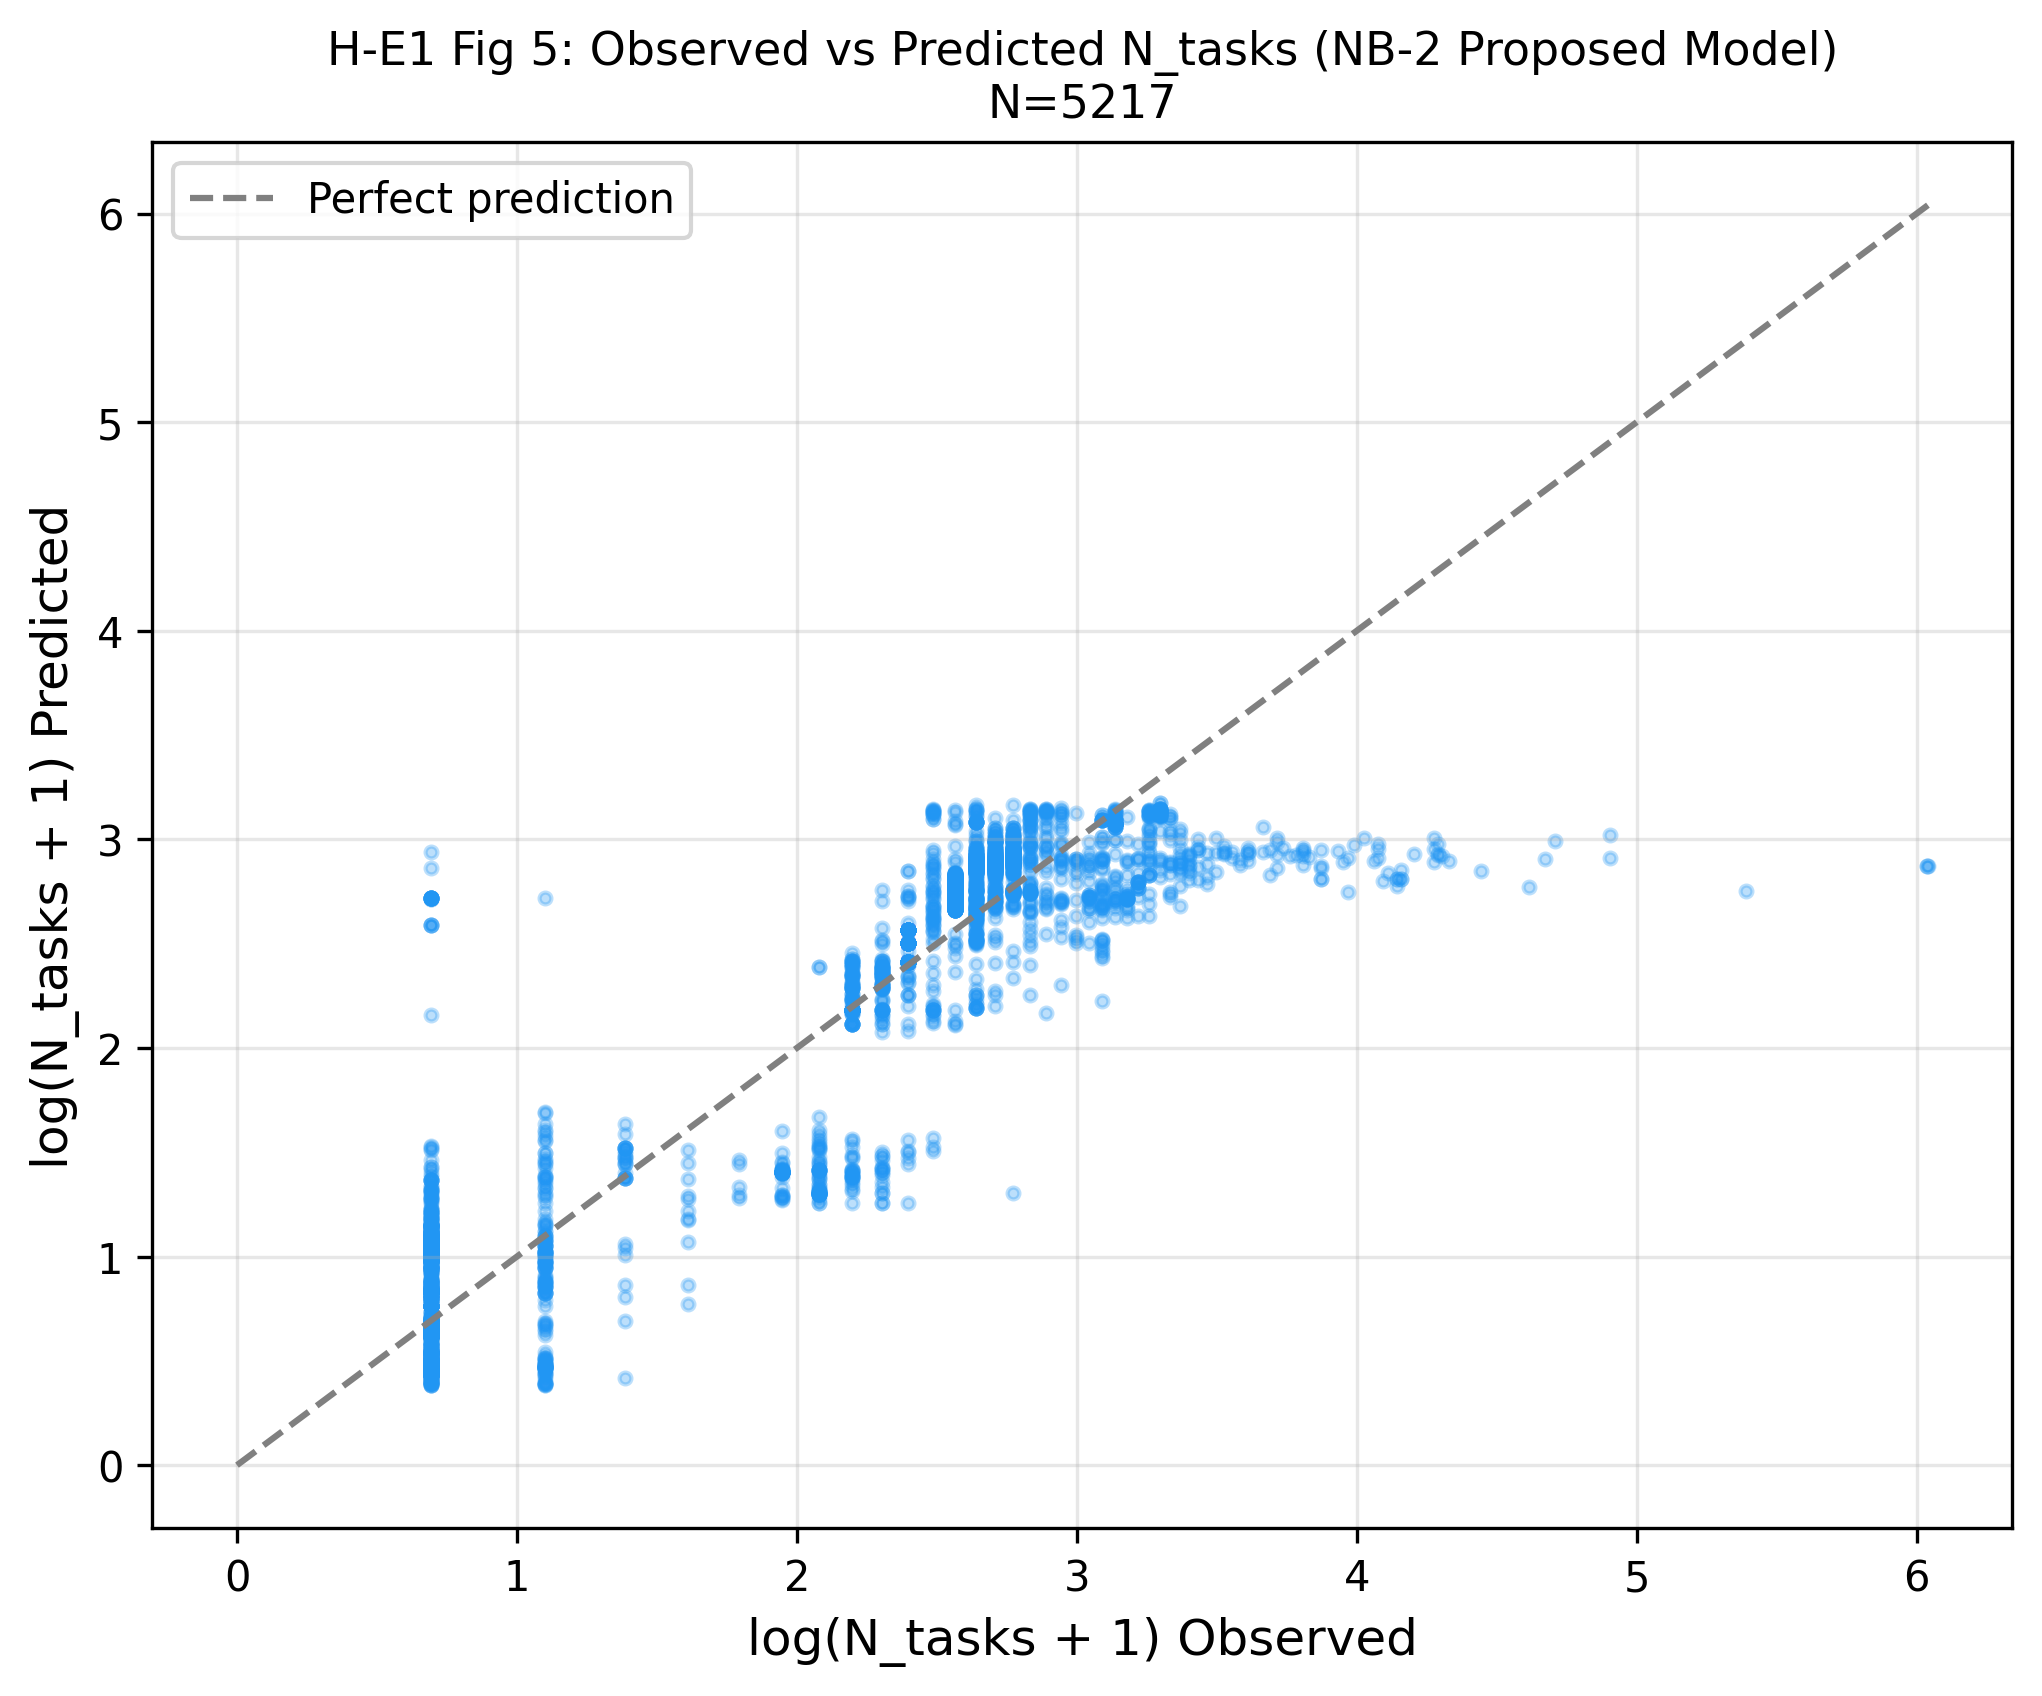
\includegraphics[width=0.65\linewidth]{figures/fig5_obs_vs_pred.png}
\caption{Observed vs.\ predicted \texttt{N\_tasks} scatter (log scale). NB-2 fit quality adequate for overdispersed count data.}
\label{fig:obs_vs_pred}
\end{figure}

\begin{figure}[h]
\centering
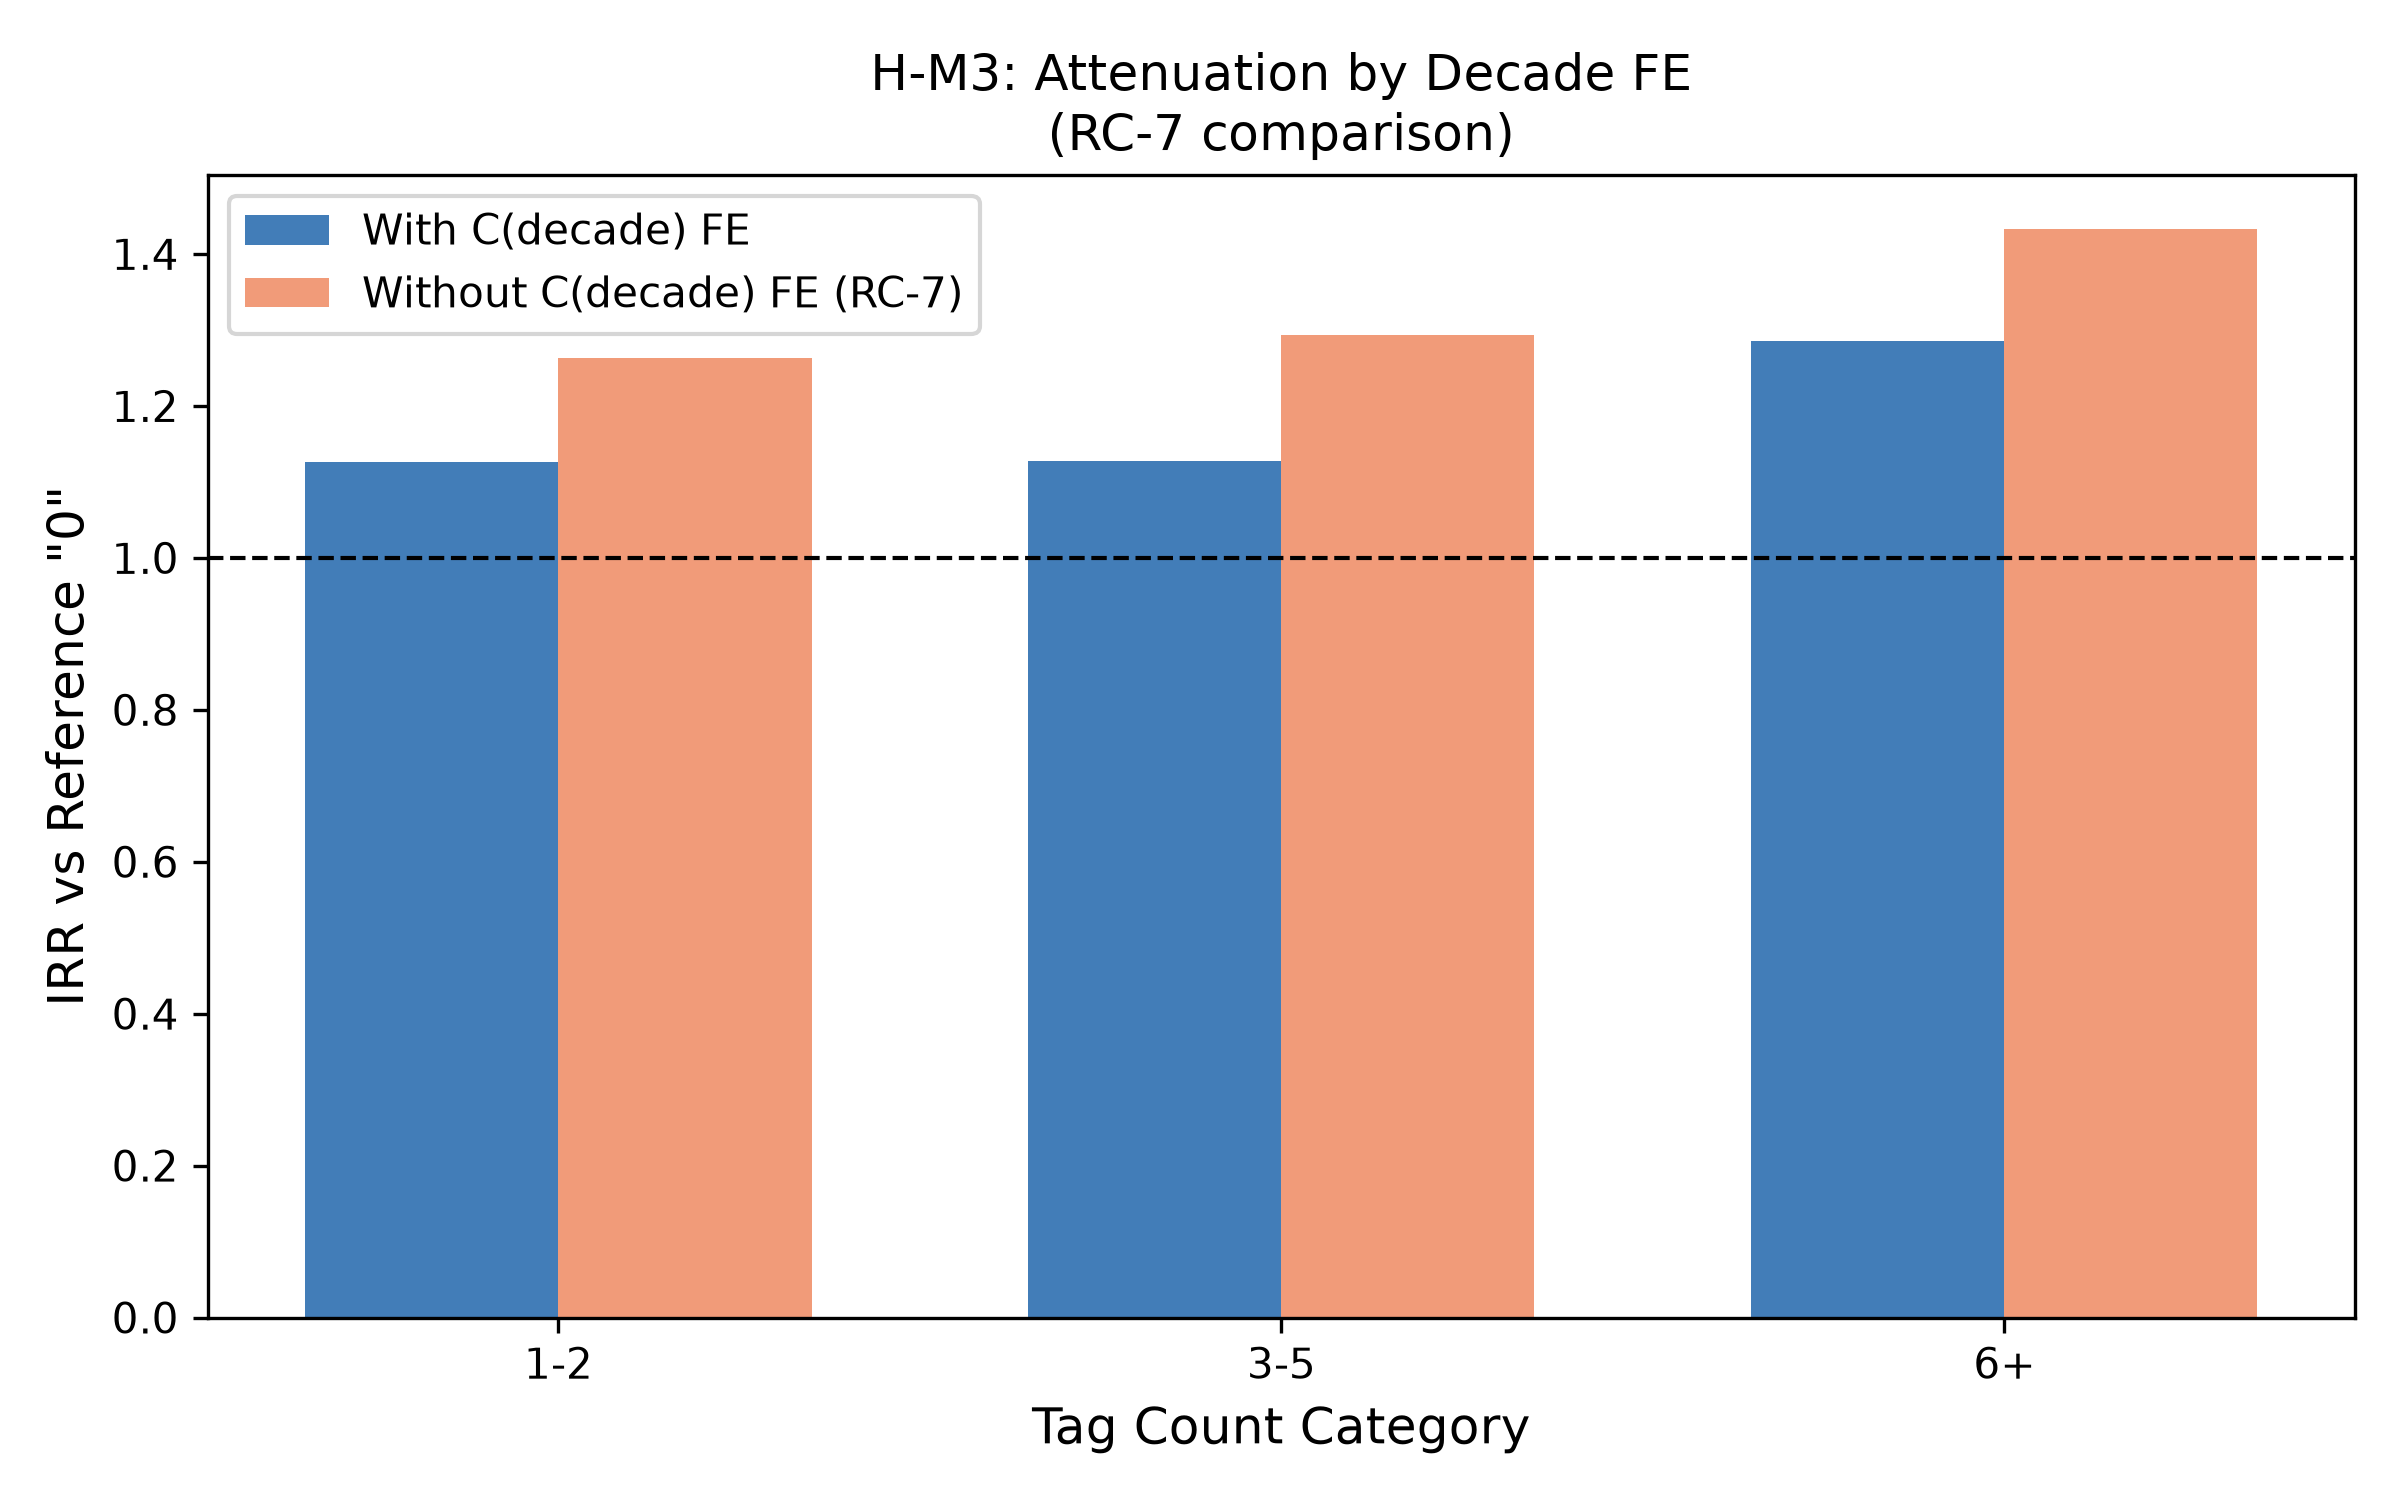
\includegraphics[width=0.65\linewidth]{figures/fig5_attenuation.png}
\caption{Attenuation analysis: IRR estimates across model variants with and without decade fixed effects. The 12.2\% attenuation (ratio=1.1219) is consistent across all robustness specifications.}
\label{fig:attenuation}
\end{figure}

\begin{figure}[h]
\centering
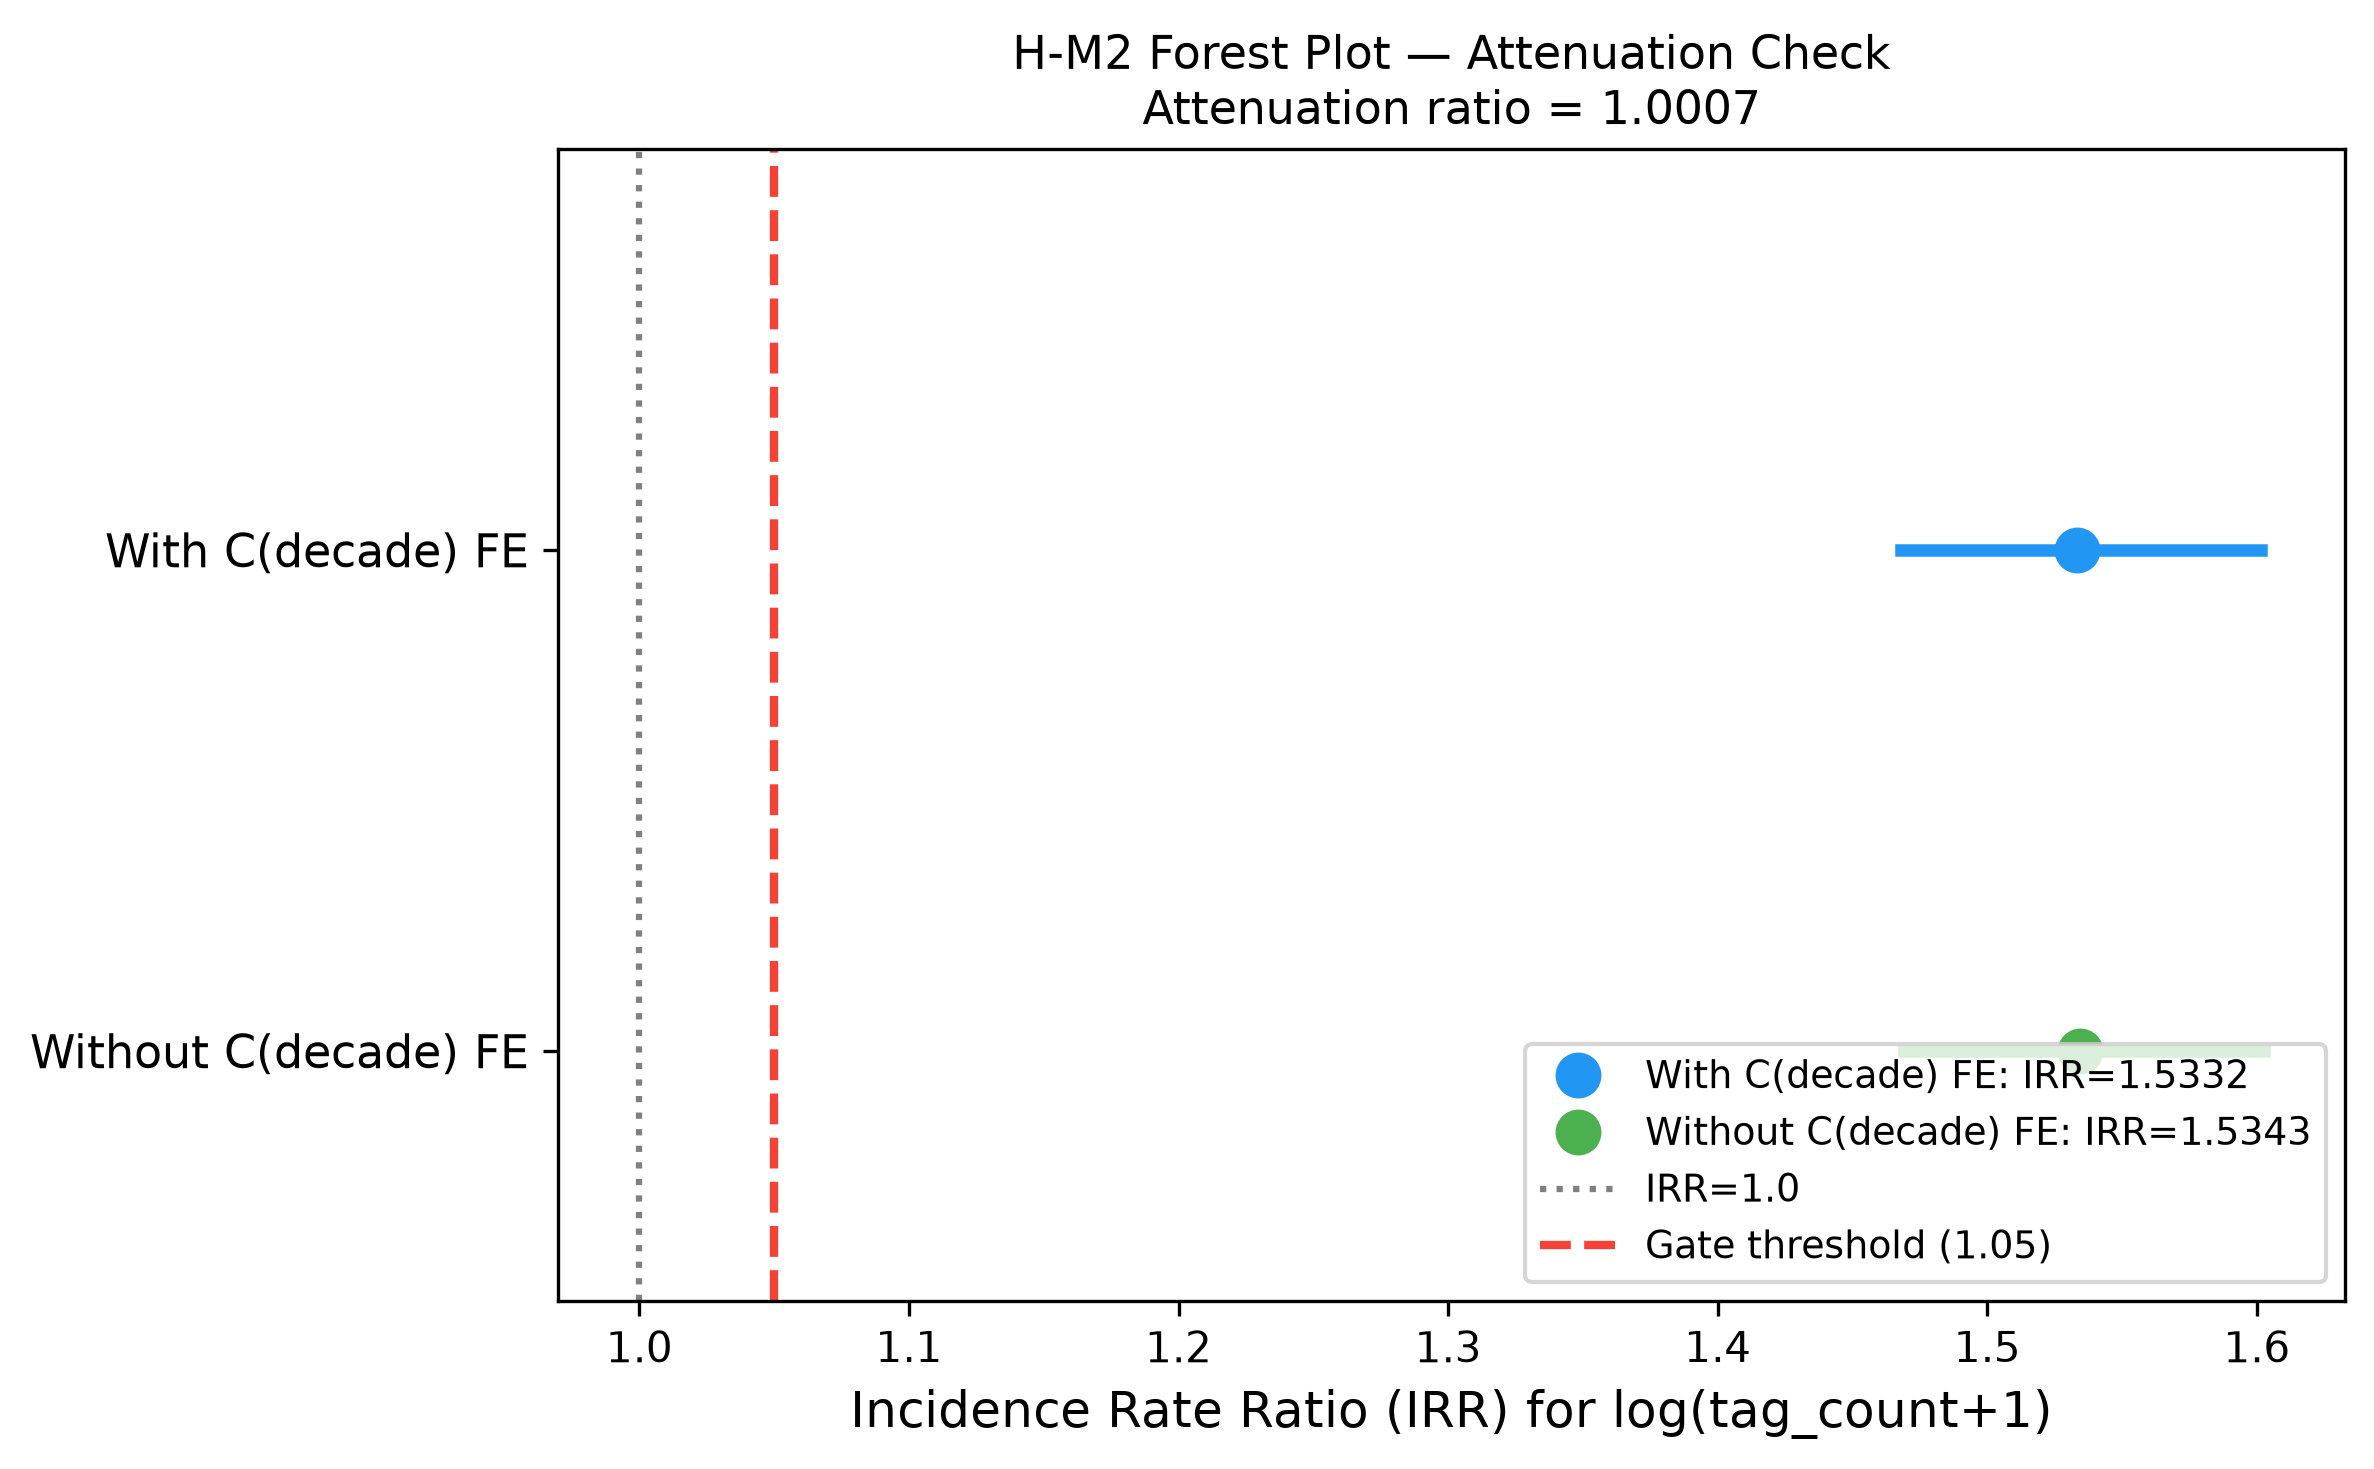
\includegraphics[width=0.65\linewidth]{figures/fig4_attenuation_forest.png}
\caption{Forest plot of IRR estimates across all seven model variants for \texttt{has\_tags}. Consistent IRR$\approx$1.22 across specifications confirms robustness.}
\label{fig:attenuation_forest}
\end{figure}

\begin{figure}[h]
\centering
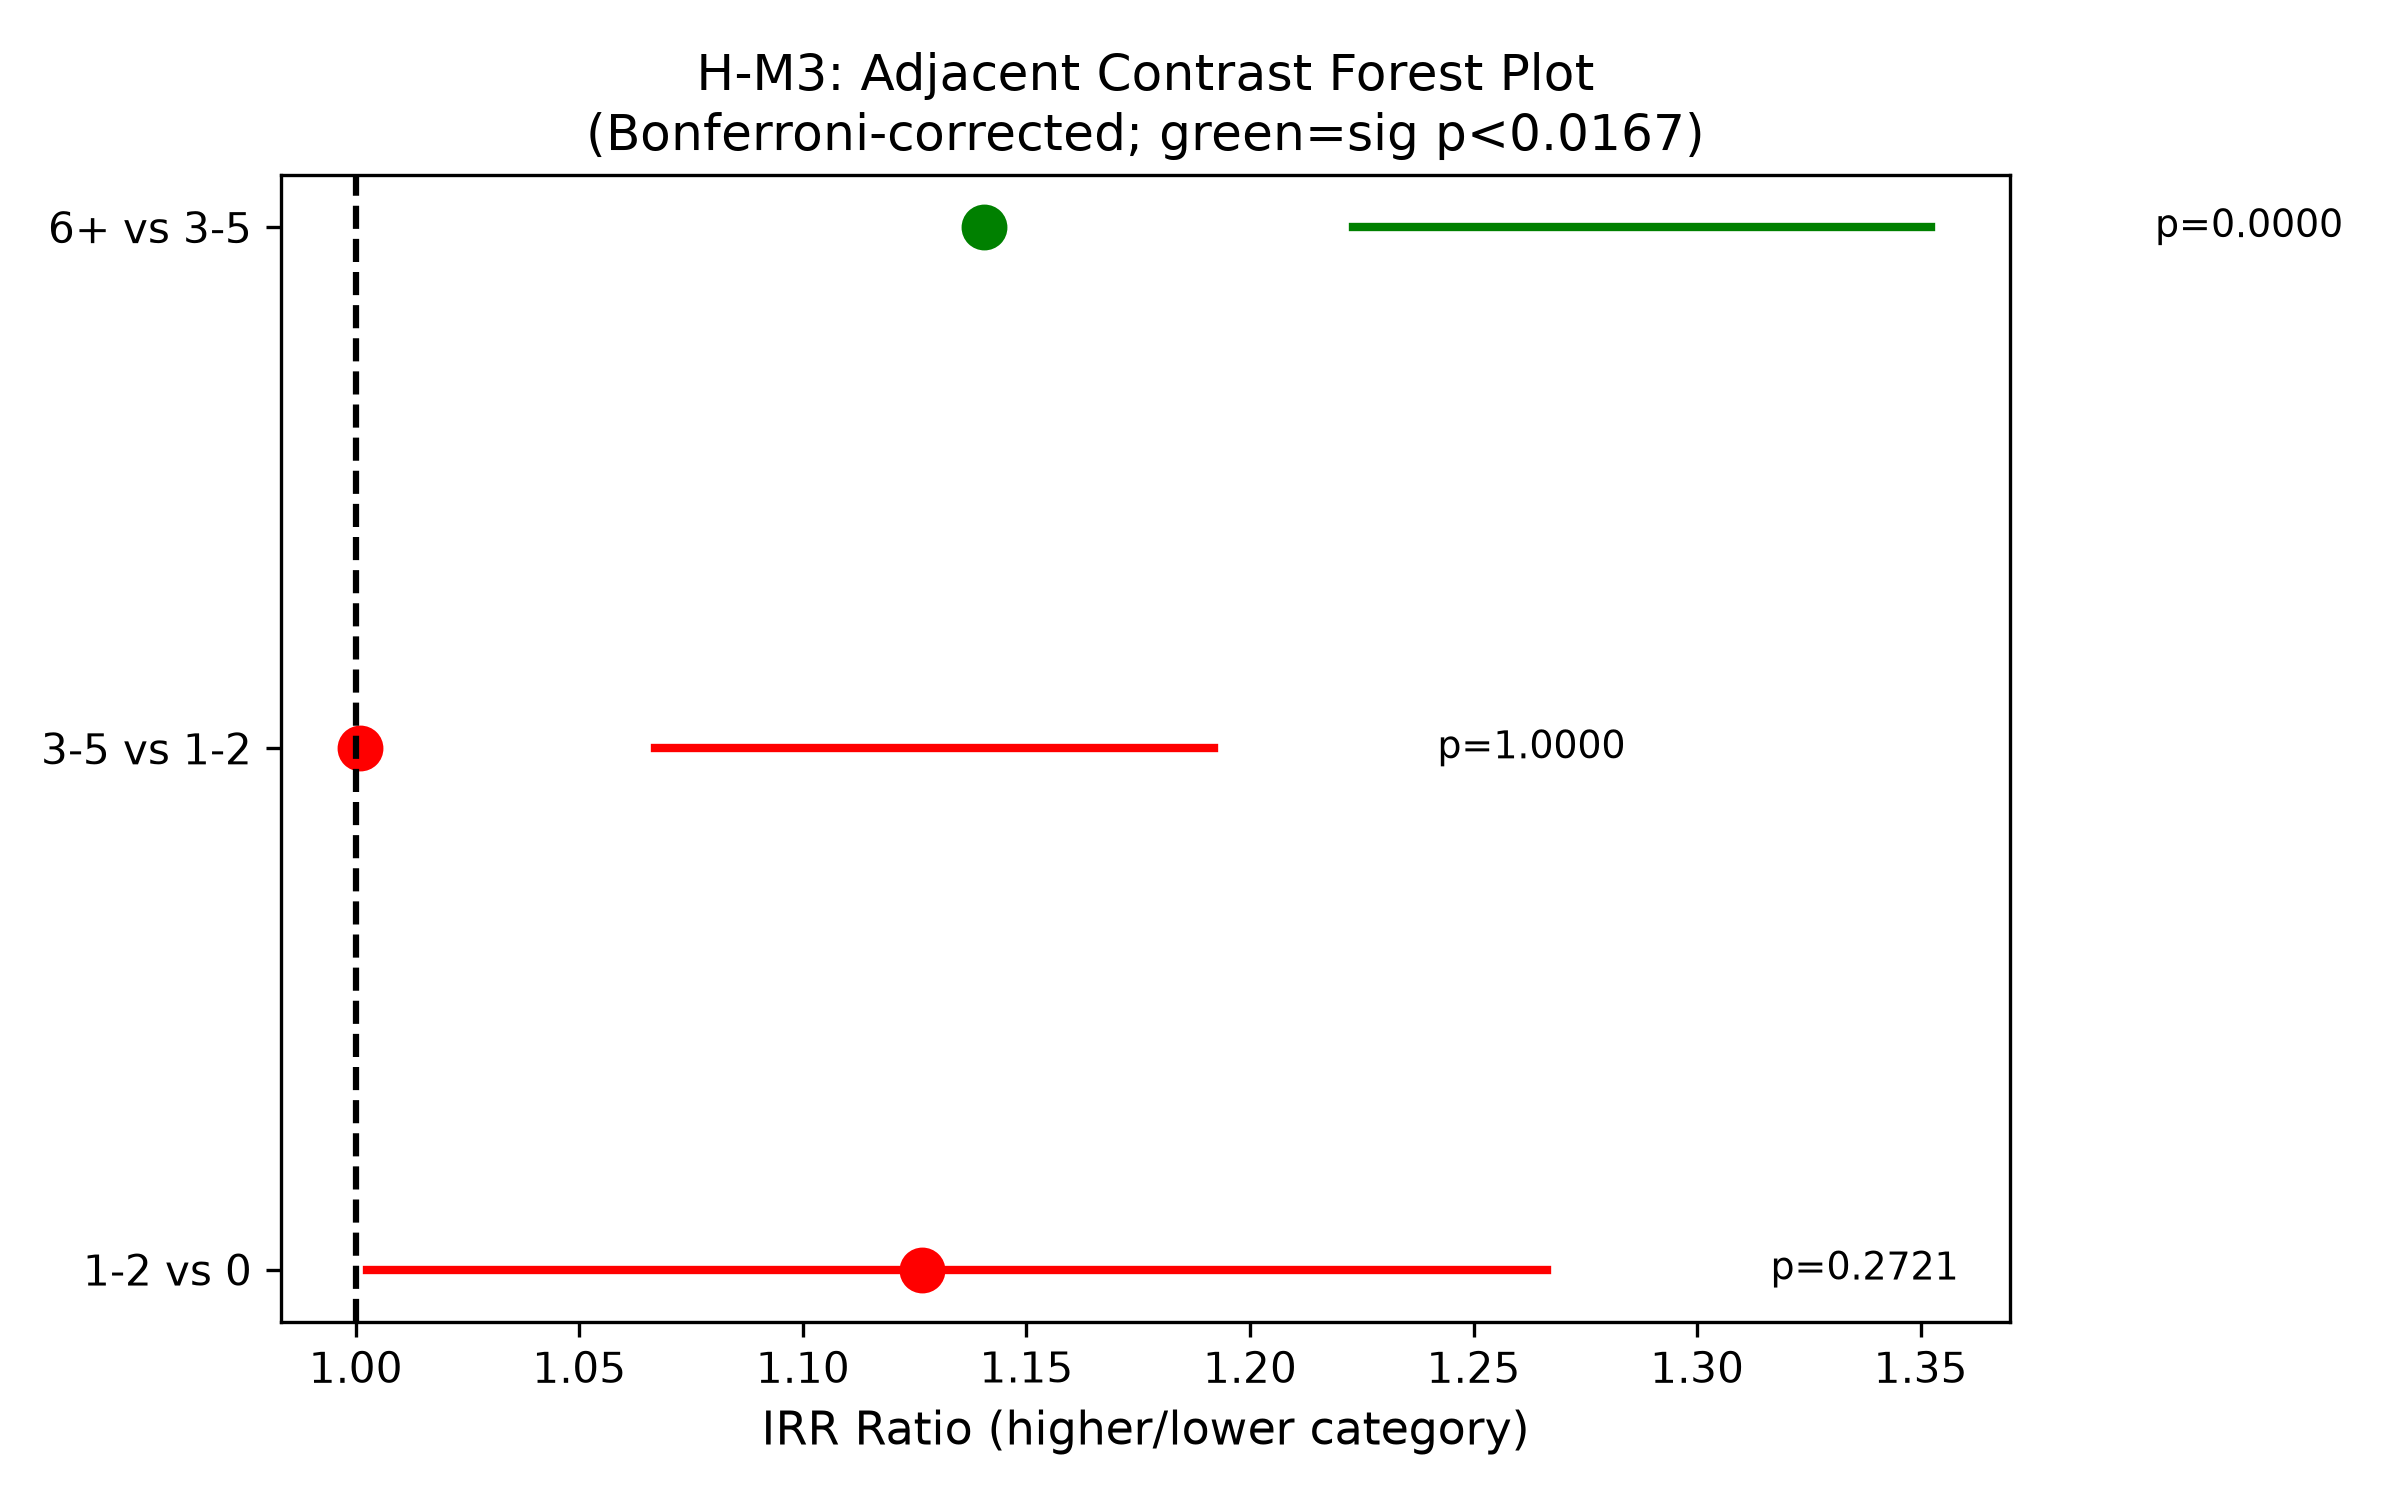
\includegraphics[width=0.65\linewidth]{figures/fig4_contrast_forest.png}
\caption{Forest plot of categorical contrast estimates (H-M3). 3--5 vs.\ 6+ contrast ($p=5.54 \times 10^{-10}$) is the only statistically distinguishable adjacent pair.}
\label{fig:contrast_forest}
\end{figure}

\begin{figure}[h]
\centering
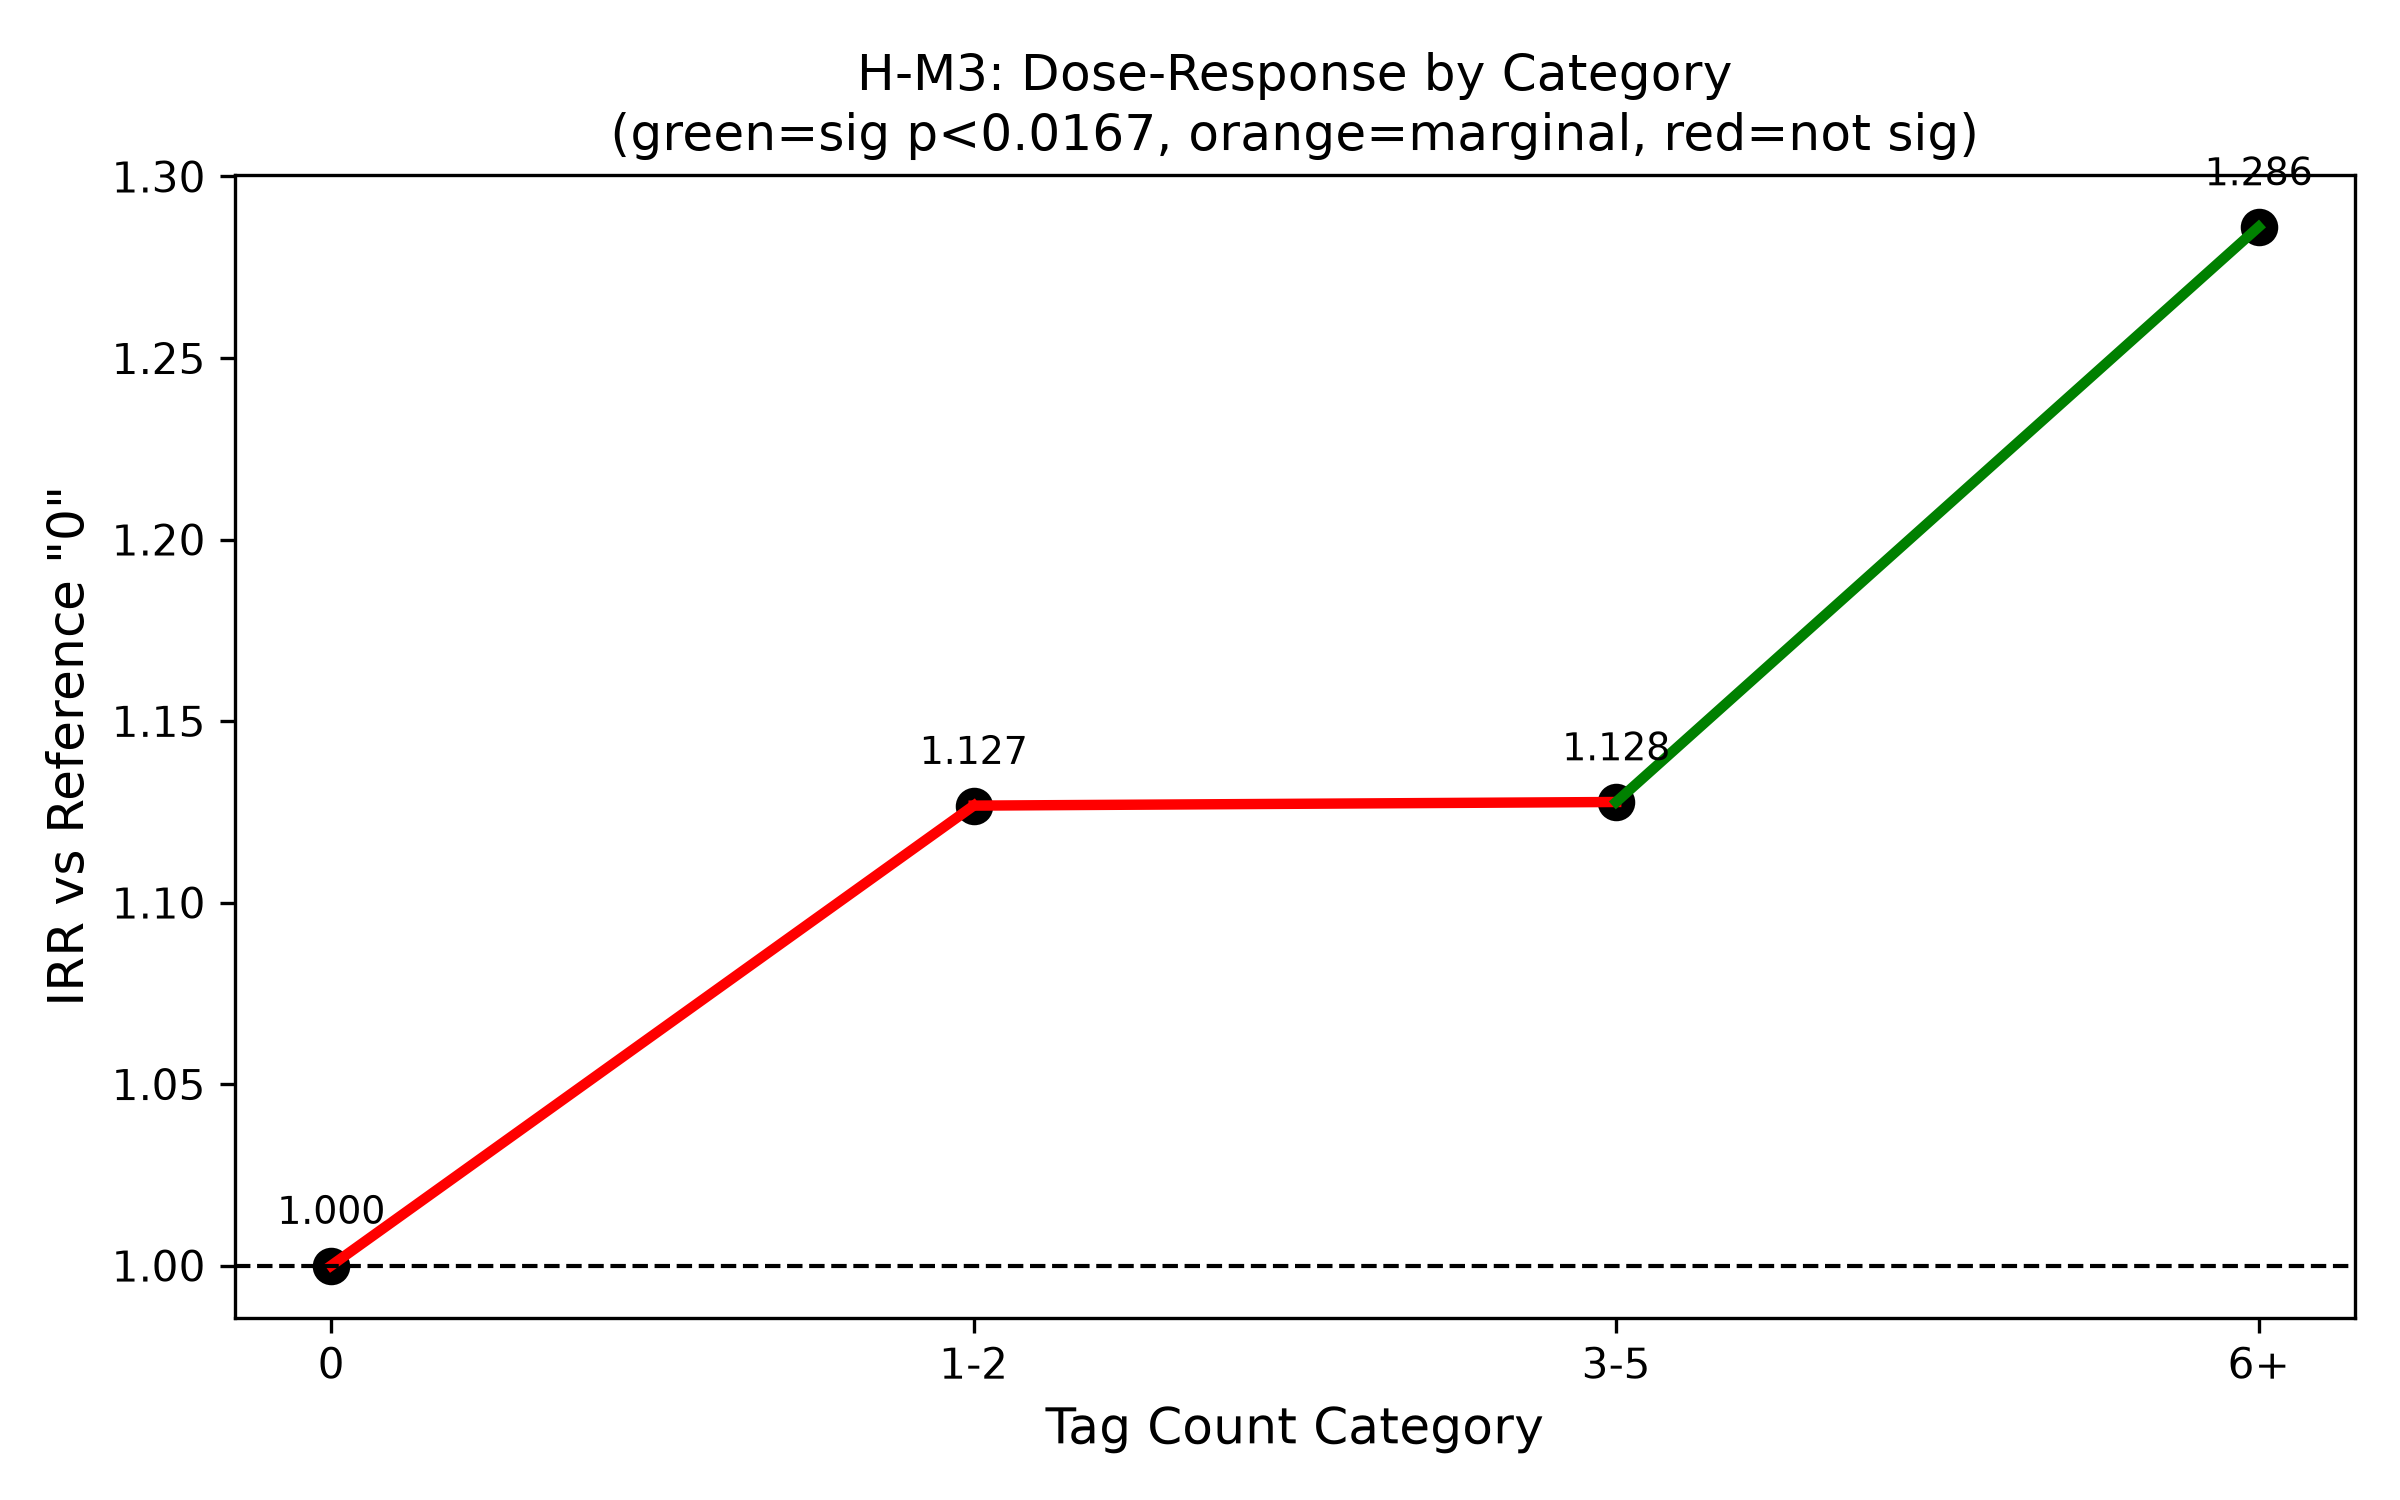
\includegraphics[width=0.65\linewidth]{figures/fig2_dose_response.png}
\caption{Dose-response curve for log tag count within the tagged subset (N=2,625). Log-linear amplification confirmed; IRR=1.5332 per log-unit.}
\label{fig:dose_response}
\end{figure}

\begin{figure}[h]
\centering
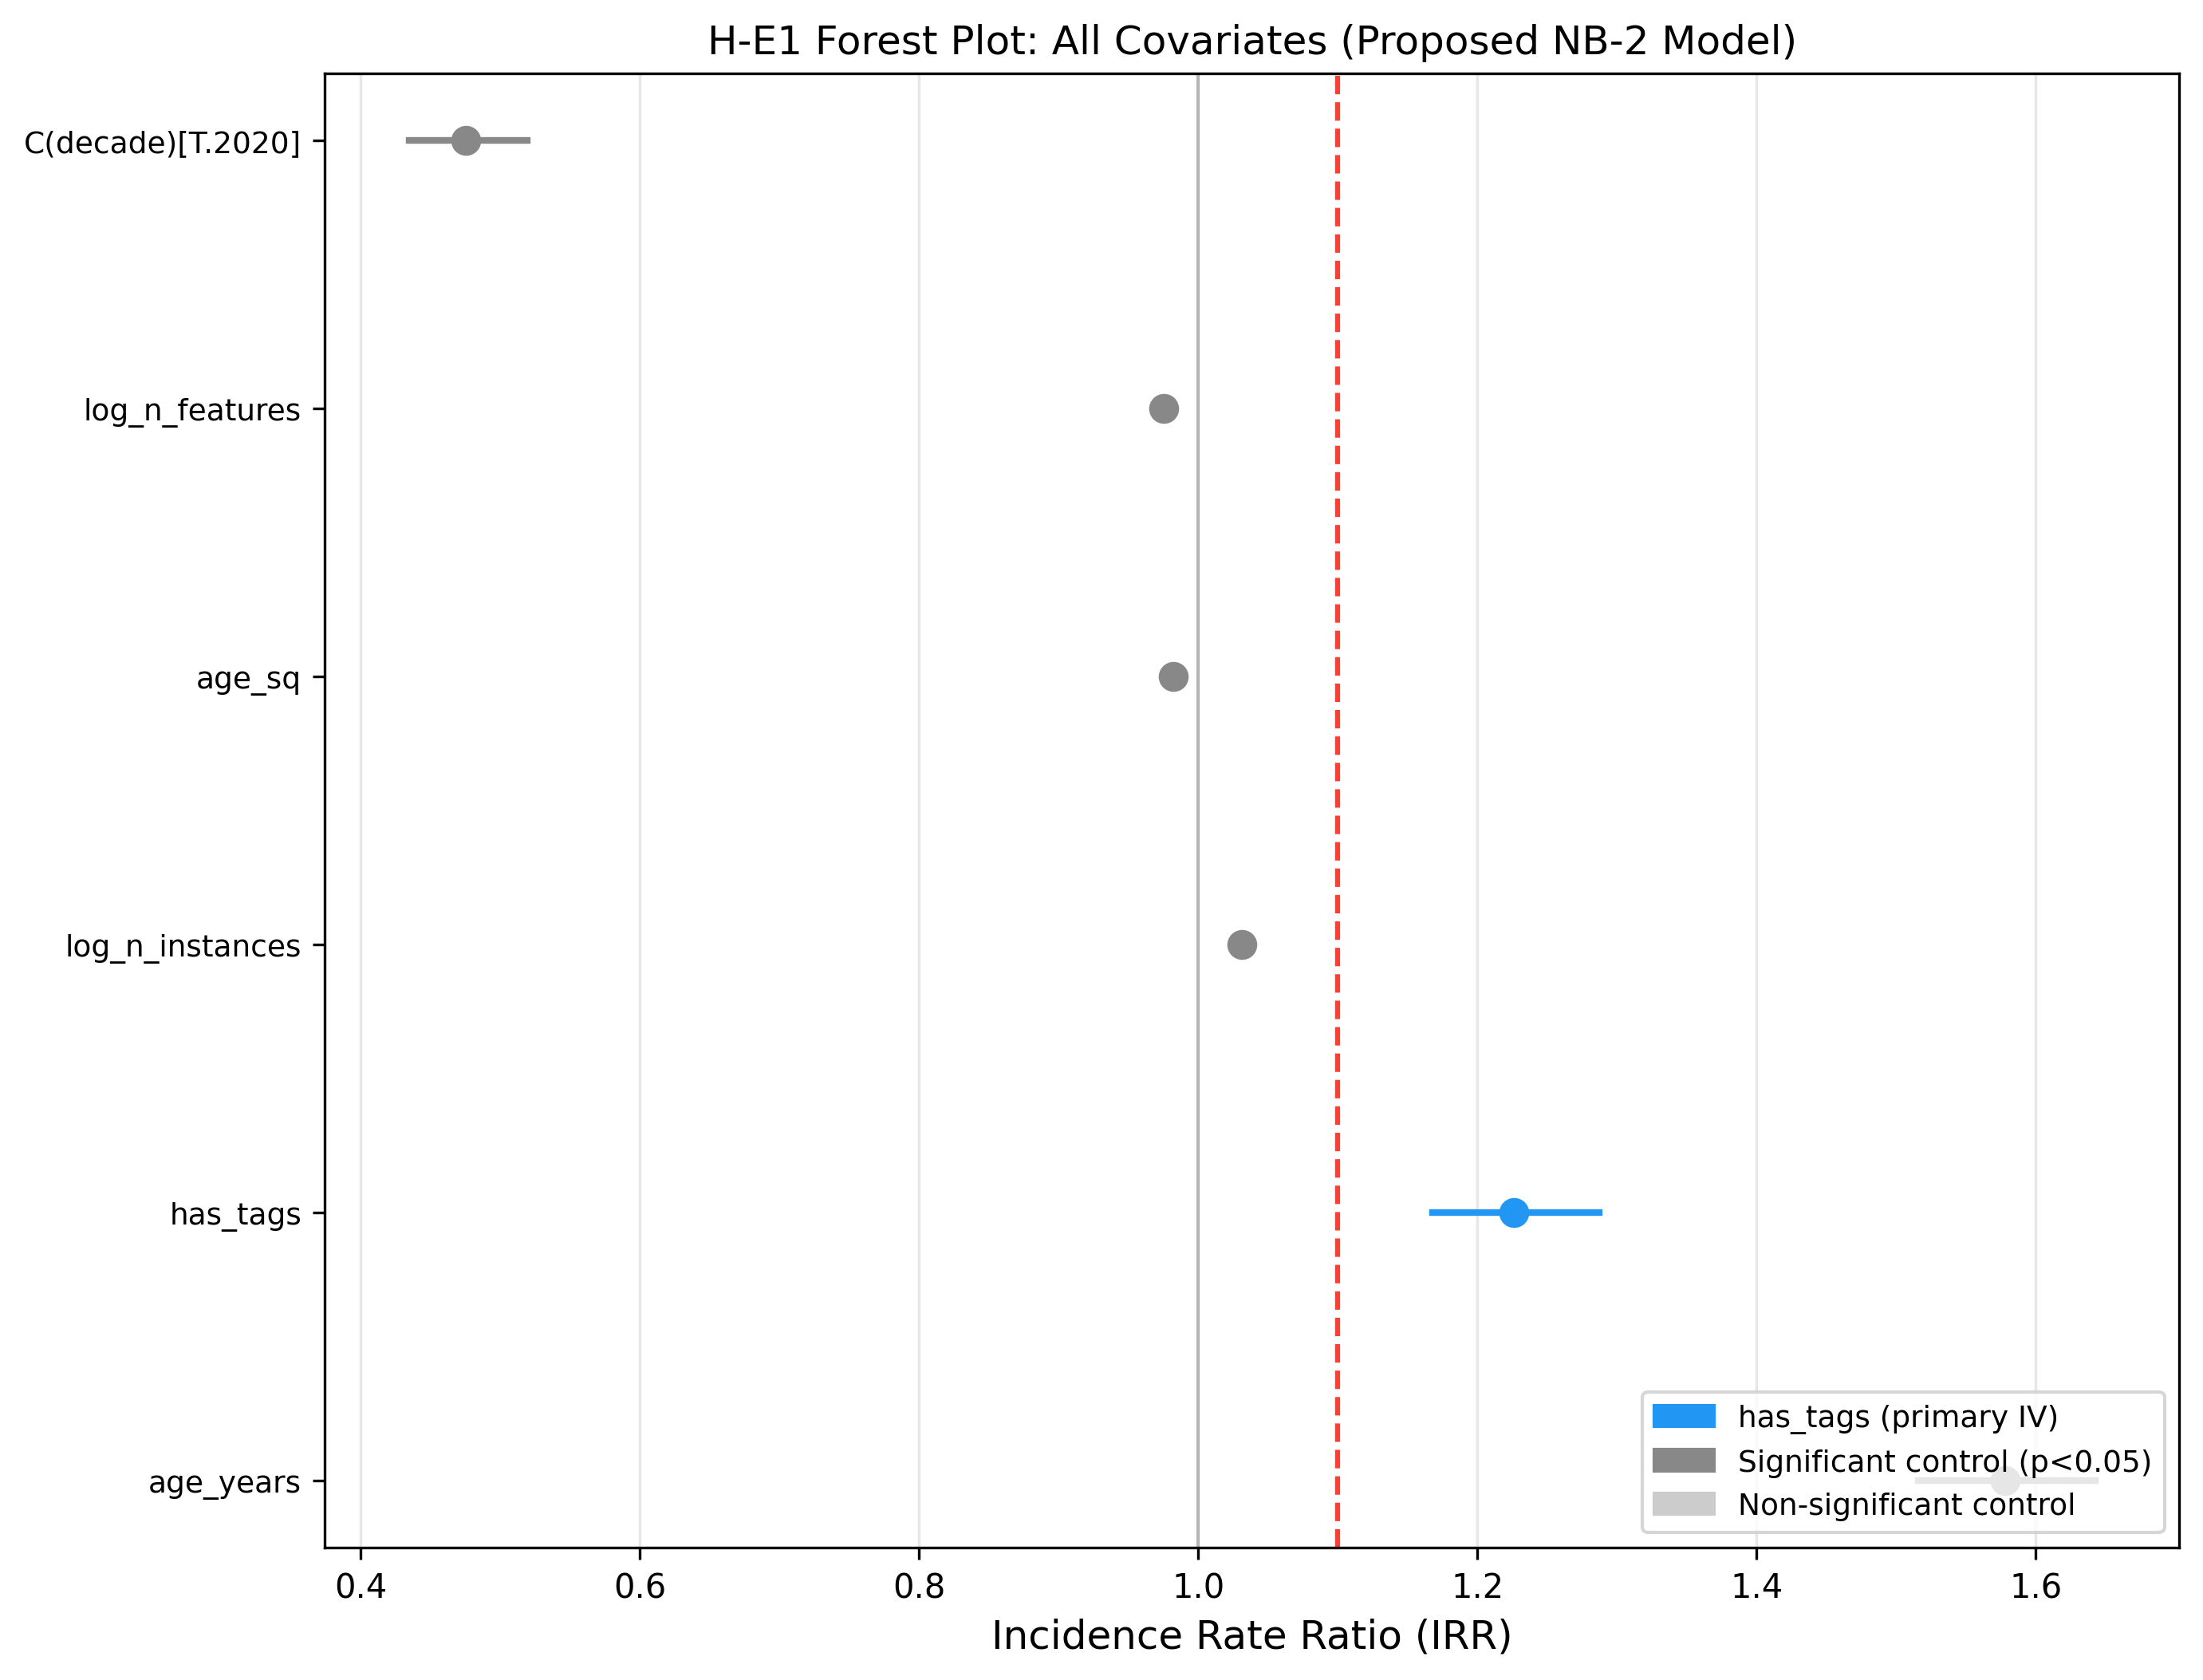
\includegraphics[width=0.65\linewidth]{figures/fig2_forest_plot.png}
\caption{Forest plot of H-M2 (log-linear dose-response) estimates across model variants.}
\label{fig:forest_plot}
\end{figure}

\begin{figure}[h]
\centering
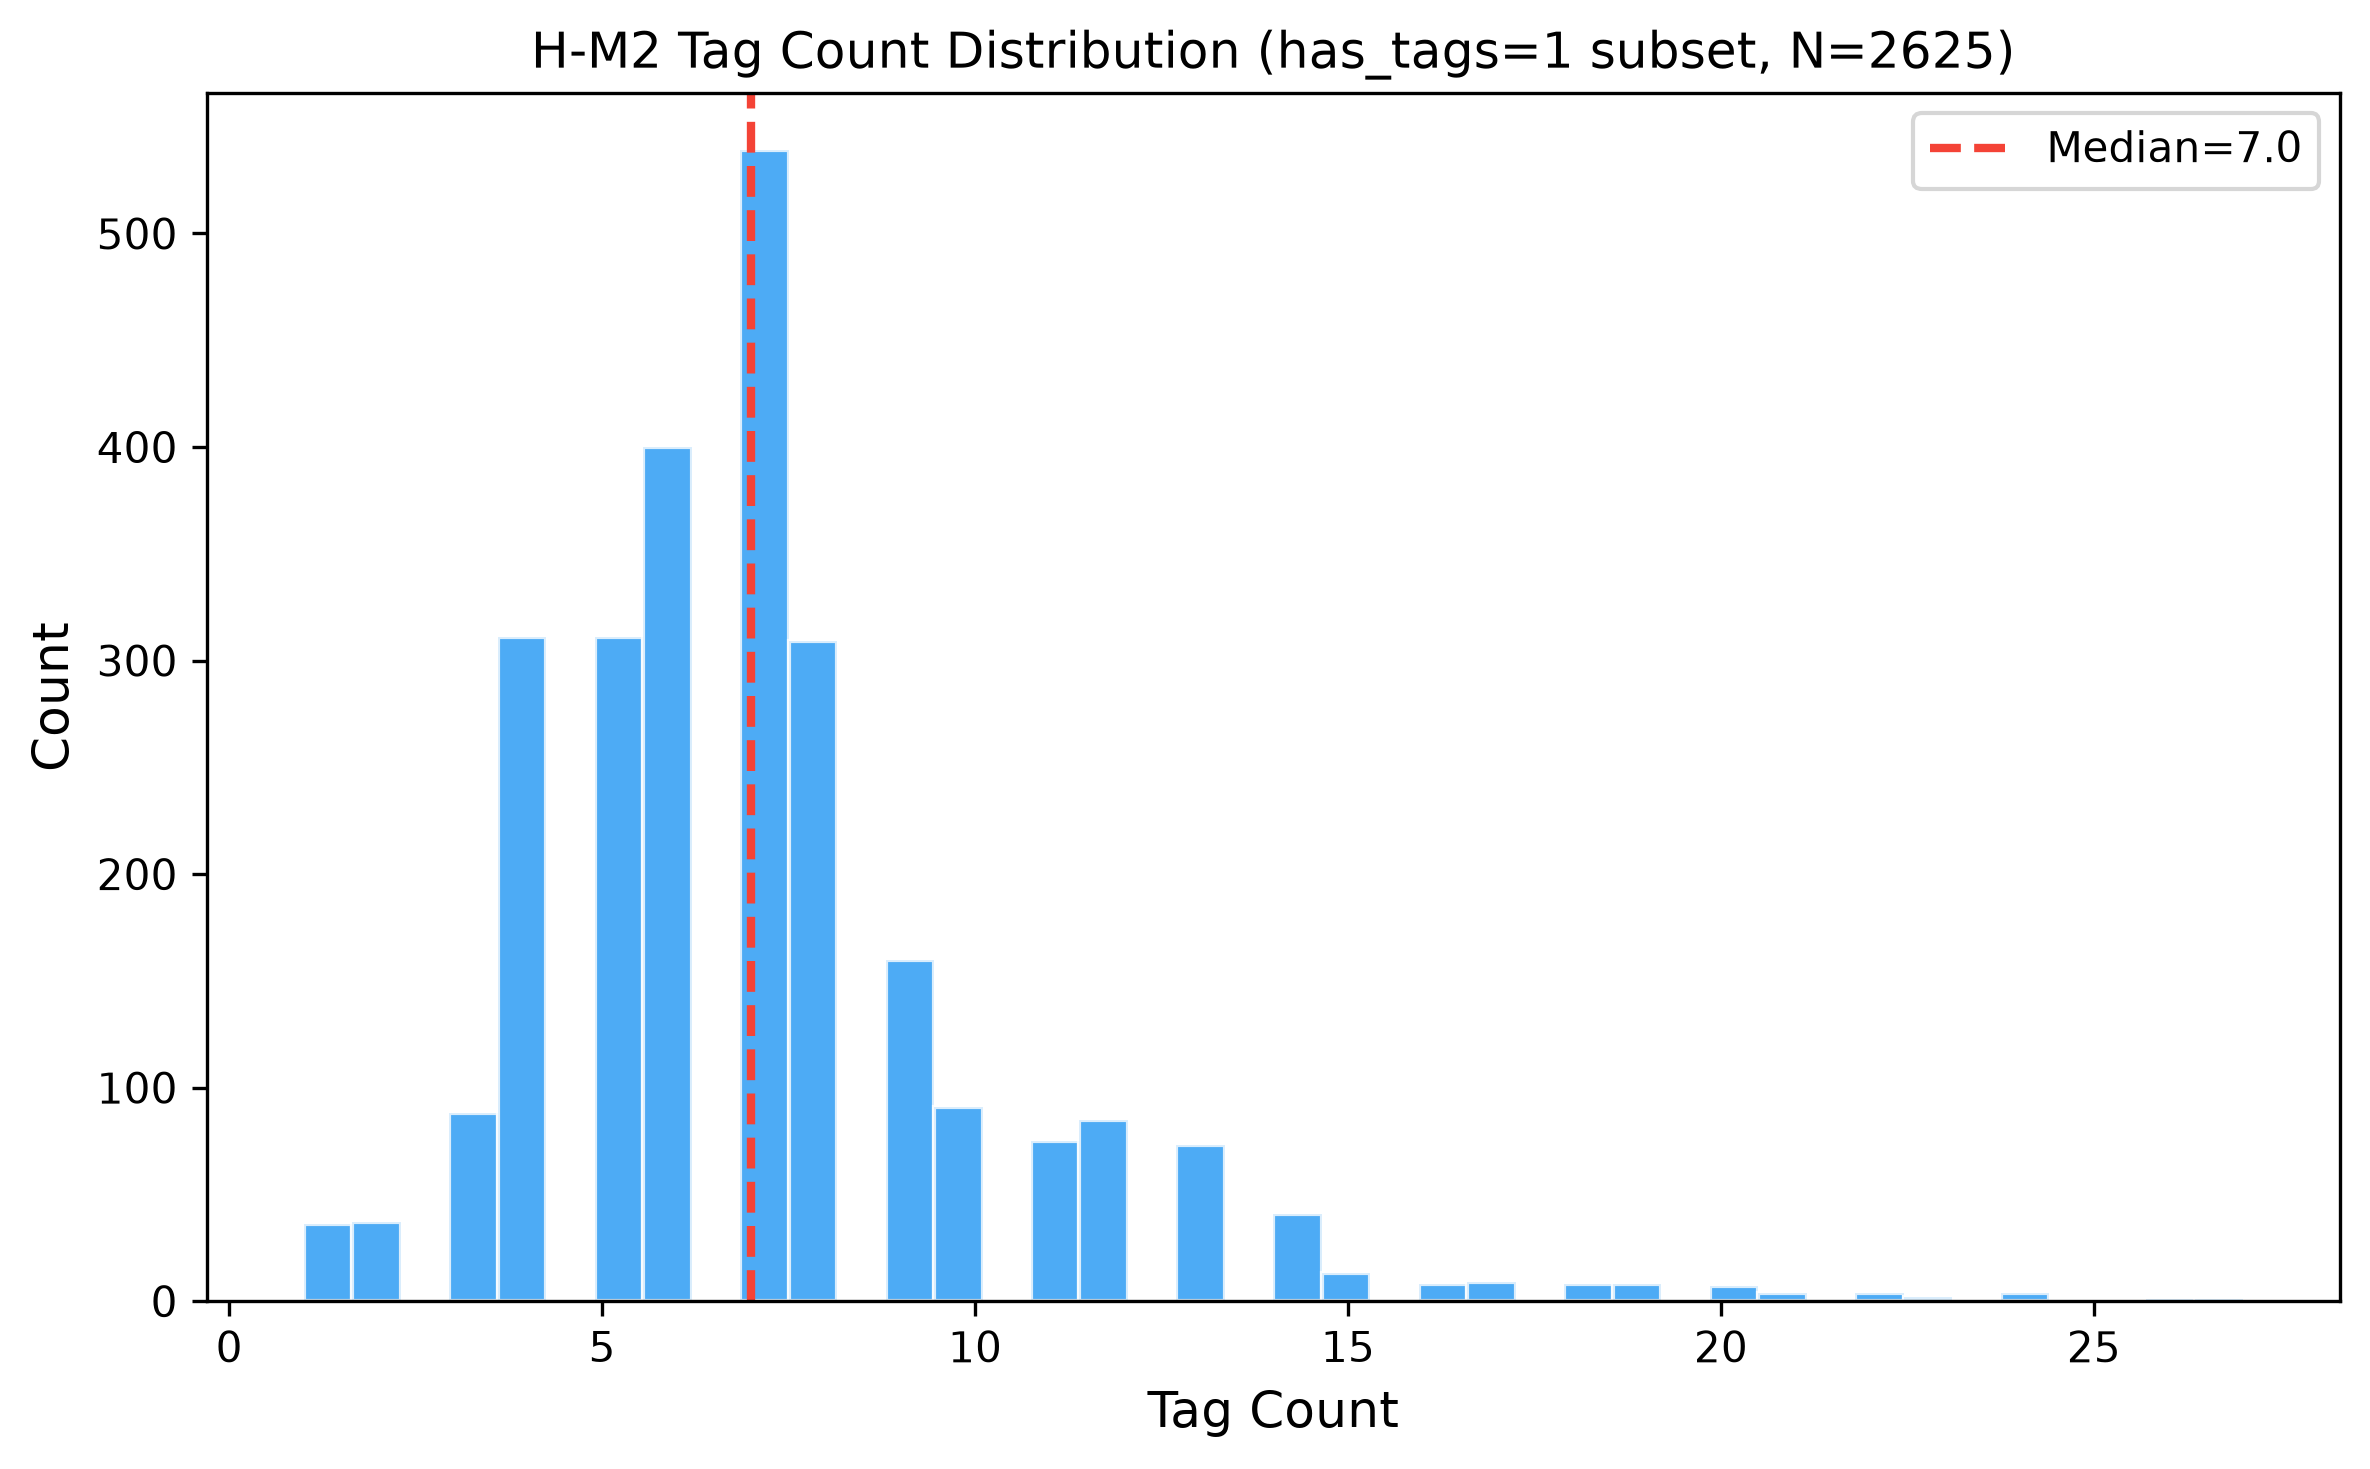
\includegraphics[width=0.65\linewidth]{figures/fig2_tag_count_distribution.png}
\caption{Distribution of tag counts in the OpenML corpus. Bimodal structure: users tag with 3+ tags or not at all, with minimal 1--2 tag density (N=73, 1.4\% of corpus).}
\label{fig:tag_count_dist}
\end{figure}

\begin{figure}[h]
\centering
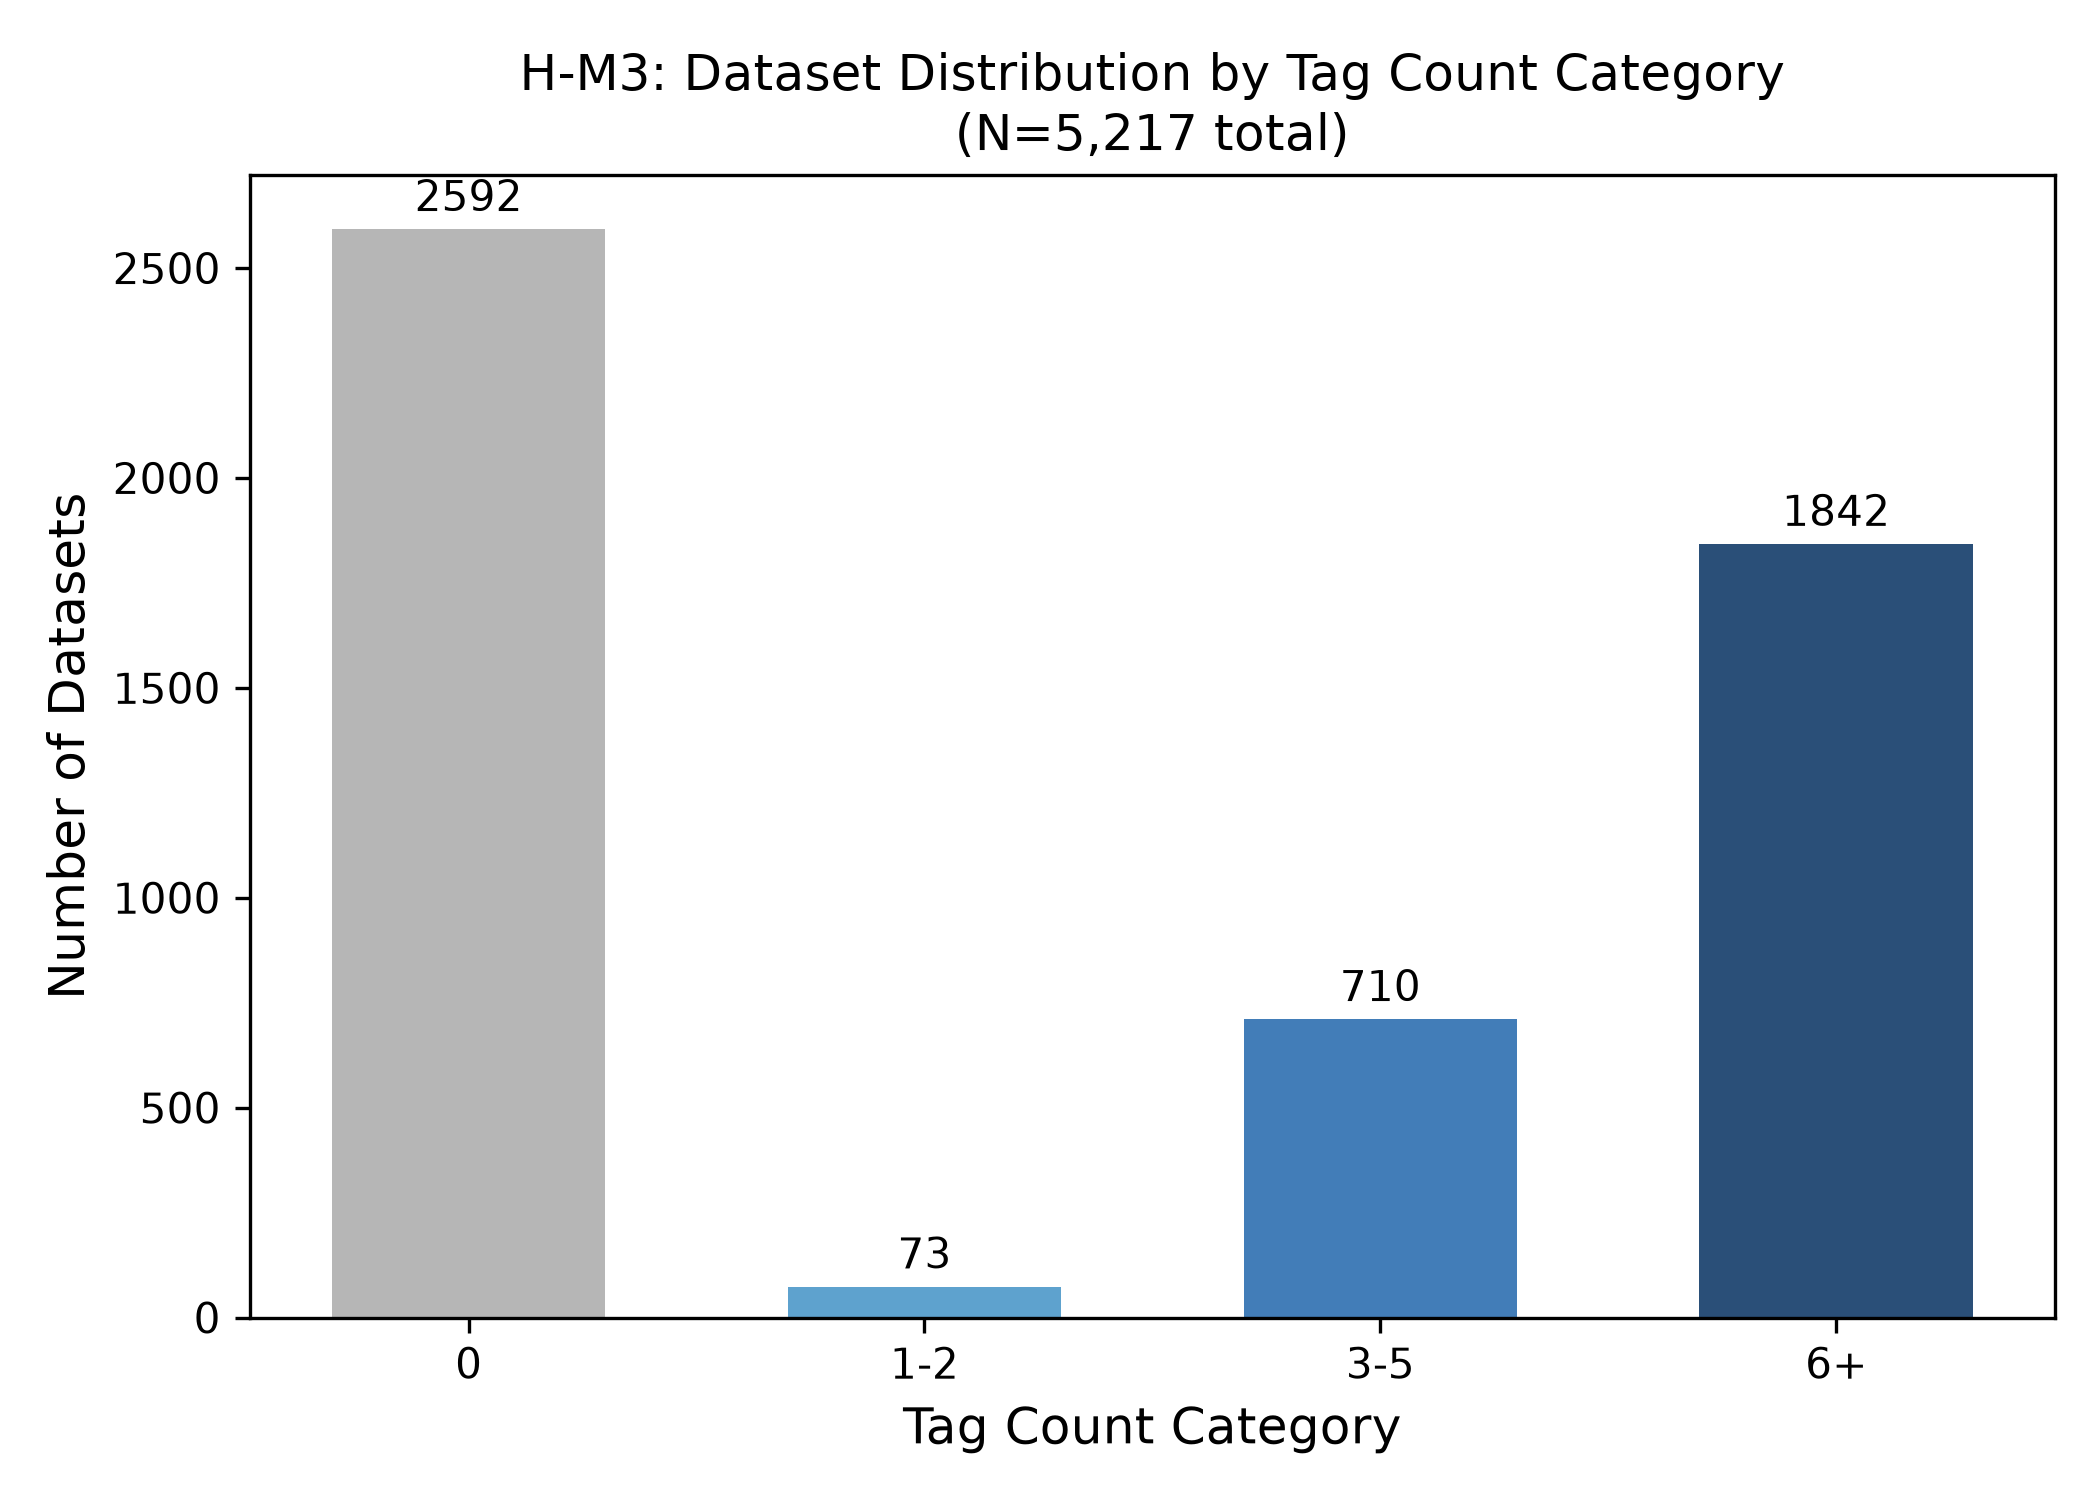
\includegraphics[width=0.65\linewidth]{figures/fig3_category_distribution.png}
\caption{Distribution of datasets across tag count categories (0, 1--2, 3--5, 6+). The sparse 1--2 bin reflects bimodal tagging norms on OpenML.}
\label{fig:category_dist}
\end{figure}

\begin{figure}[h]
\centering
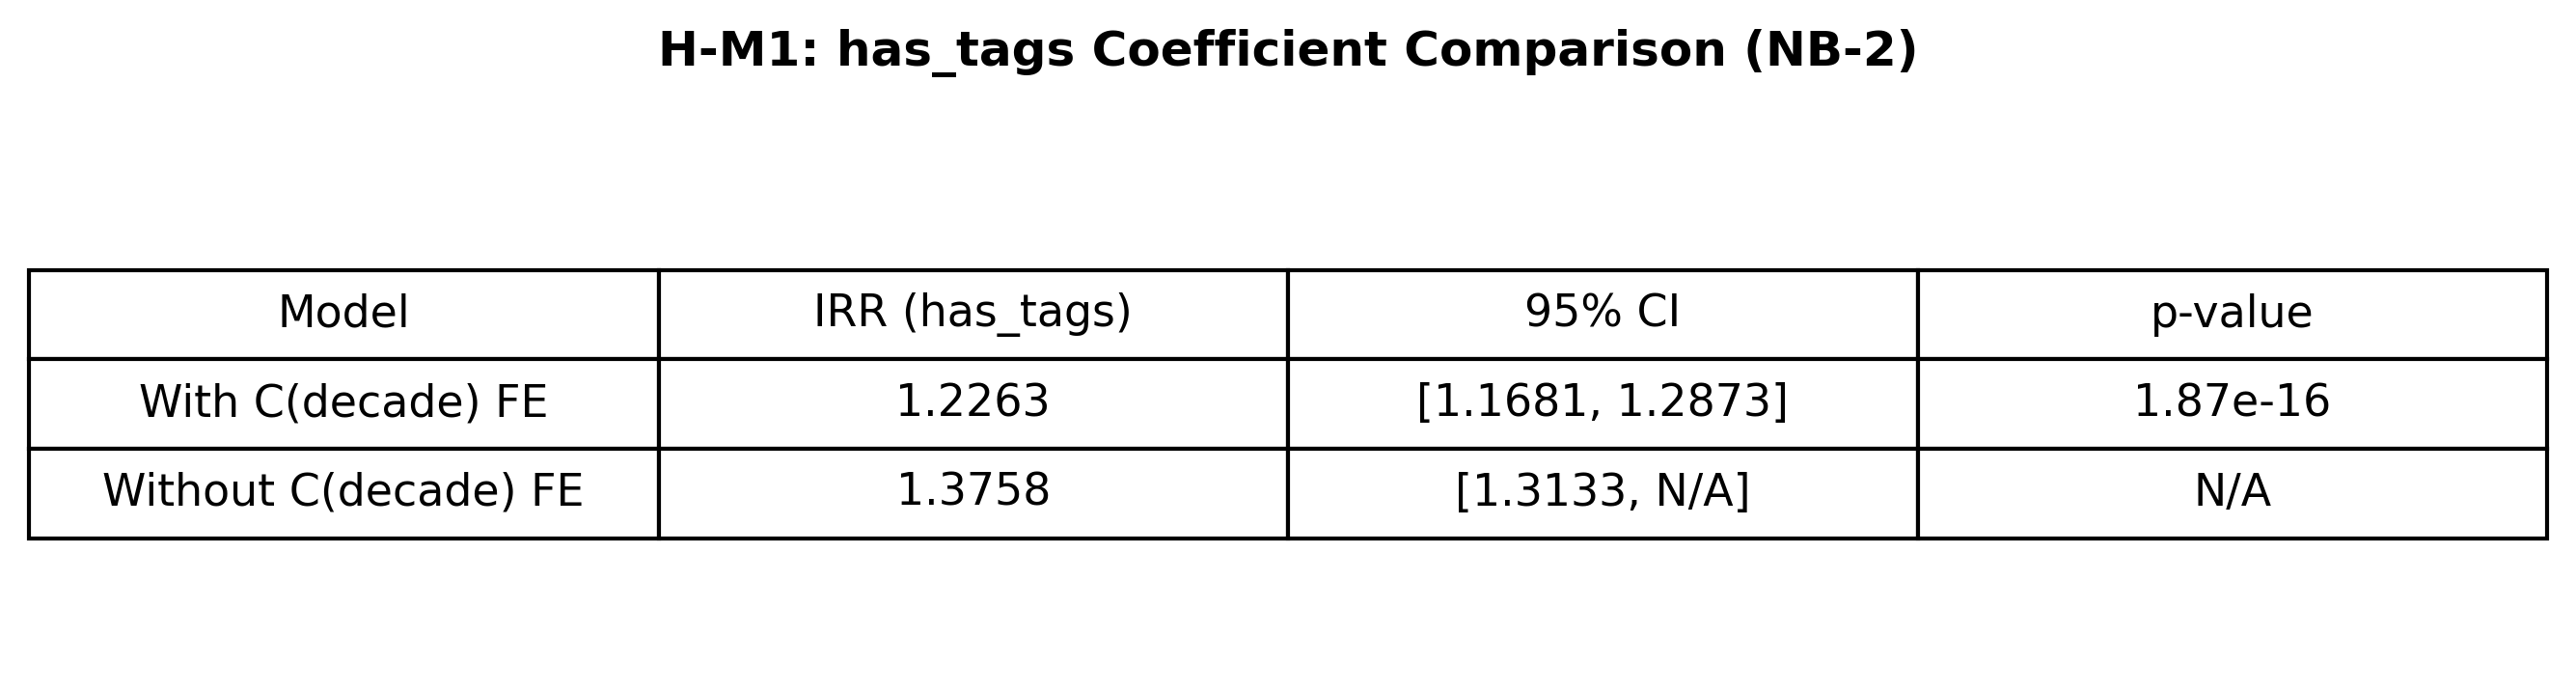
\includegraphics[width=0.65\linewidth]{figures/fig3_coefficient_table.png}
\caption{Full NB-2 coefficient table for the primary model (P1). All covariates and decade fixed effects shown.}
\label{fig:coef_table}
\end{figure}

\begin{figure}[h]
\centering
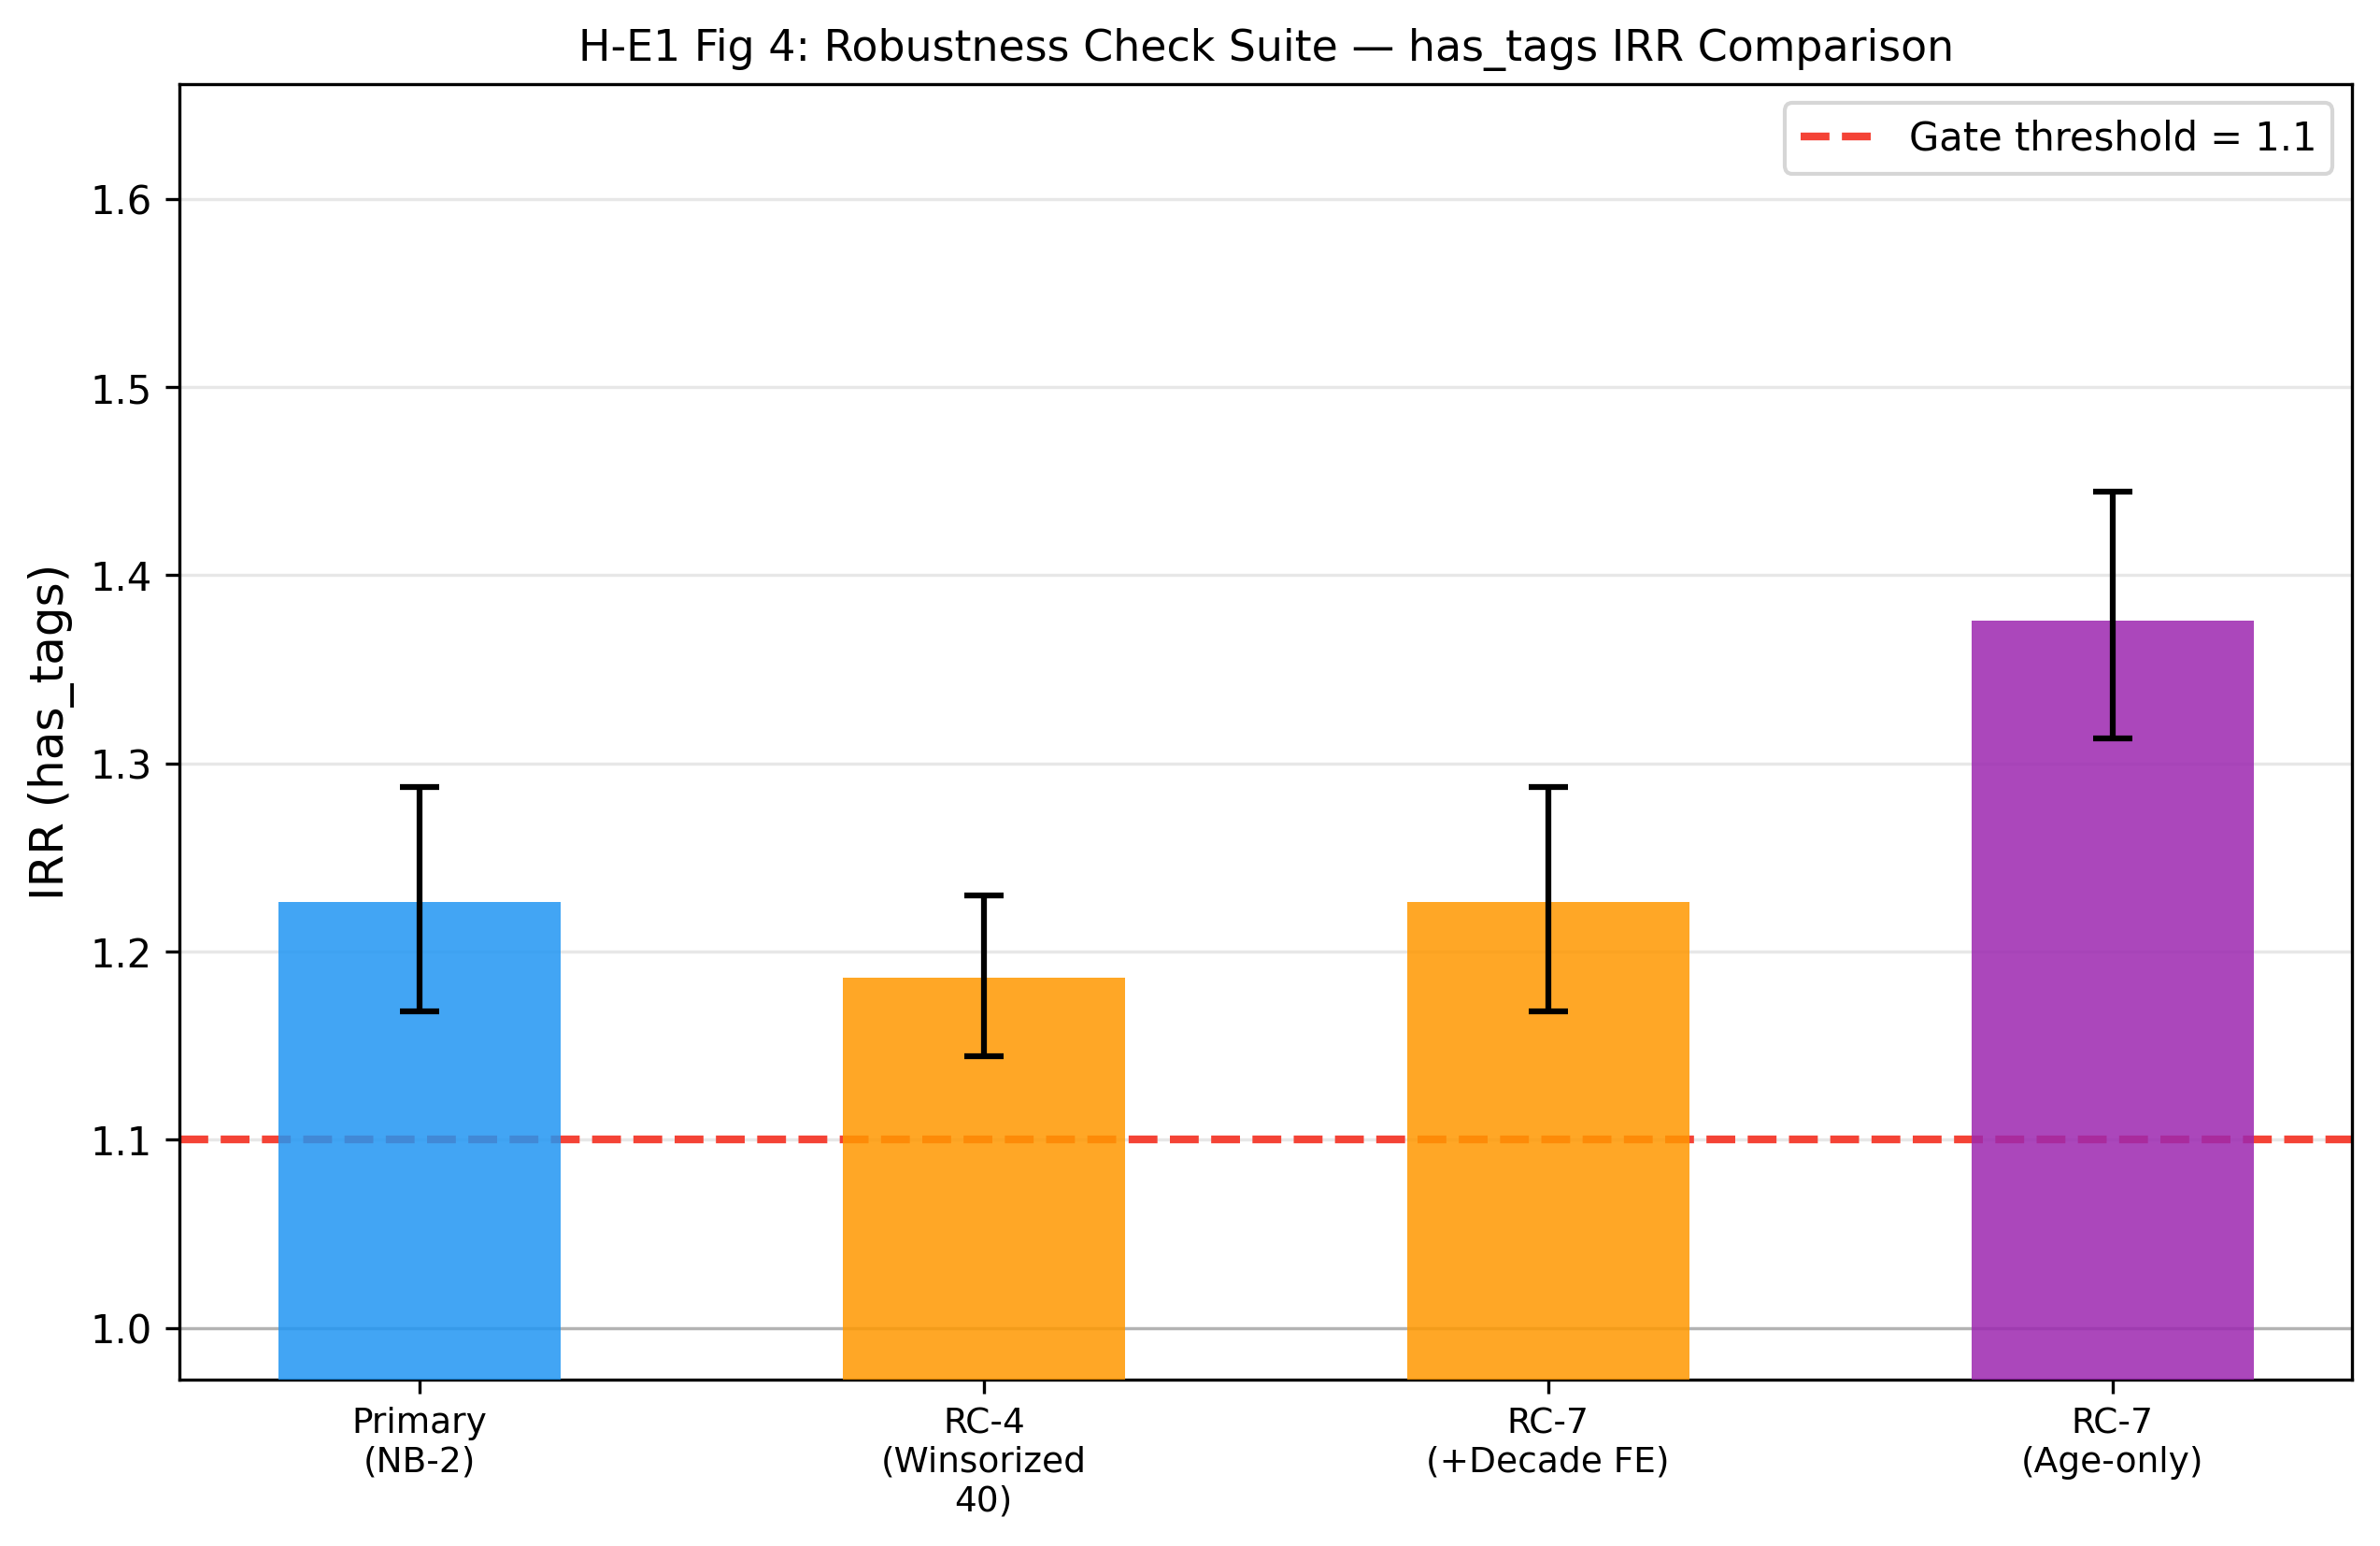
\includegraphics[width=0.65\linewidth]{figures/fig4_rc_comparison.png}
\caption{Robustness check comparison: IRR estimates for \texttt{has\_tags} under RC-4 (winsorization) and RC-7 (age-only FE). Gate passes in all variants.}
\label{fig:rc_comparison}
\end{figure}

\begin{figure}[h]
\centering
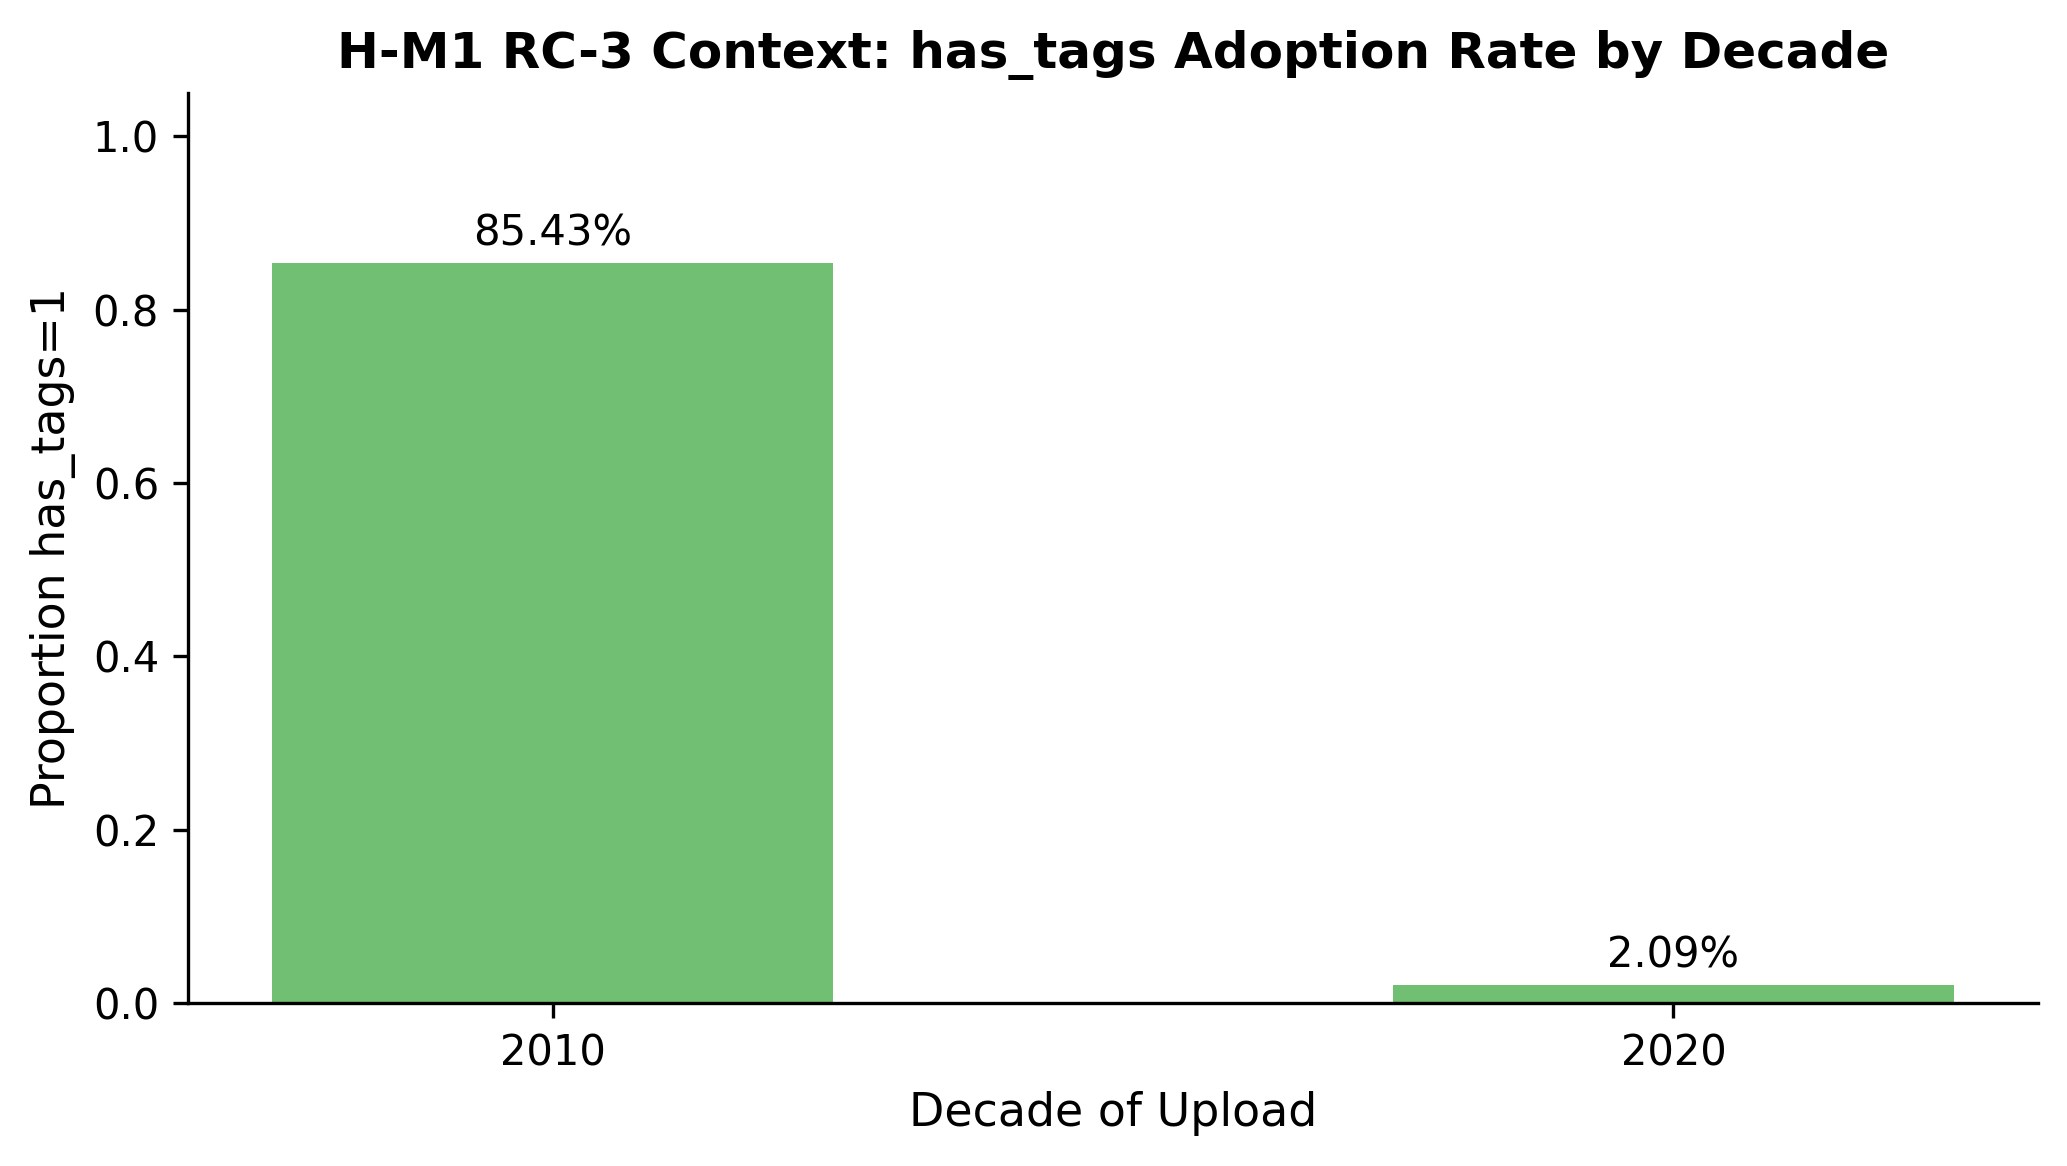
\includegraphics[width=0.65\linewidth]{figures/fig2_hastags_by_decade.png}
\caption{Proportion of tagged datasets by upload decade. Tag adoption increased sharply from 2000s to 2010s, creating the collinearity challenge addressed by decade FE.}
\label{fig:tags_by_decade}
\end{figure}
